%----------
%   WARNING
%----------

% This Guide contains Library recommendations based mainly on APA and IEEE styles, but you must always follow the guidelines of your TFG Tutor and the TFG regulations for your degree.

% THIS TEMPLATE IS BASED ON THE IEEE STYLE 

% TFG - Machine Learning Based Predictive Modeling of Energy Prices

%----------
% DOCUMENT SETTINGS
%----------

\documentclass[12pt]{report} % font: 12pt

% margins: 2.5 cm top and bottom; 3 cm left and right
\usepackage[
a4paper,
vmargin=2.5cm,
hmargin=3cm
]{geometry}

% Paragraph Spacing and Line Spacing: Narrow (6 pt / 1.15 spacing) or Moderate (6 pt / 1.5 spacing)
\renewcommand{\baselinestretch}{1.15}
\parskip=6pt

% Color settings for cover and code listings 
\usepackage[table]{xcolor}
\definecolor{azulUC3M}{RGB}{0,0,102}
\definecolor{gray97}{gray}{.97}
\definecolor{gray75}{gray}{.75}
\definecolor{gray45}{gray}{.45}

% PDF/A -- Important for its inclusion in e-Archive. PDF/A is the optimal format for preservation and for the generation of metadata: http://uc3m.libguides.com/ld.php?content_id=31389625.

% In the template we include the file OUTPUT.XMPDATA. You can download that file and include the metadata that will be incorporated into the PDF file when you compile the memoria.tex file. Then upload it back to your project.
\usepackage[a-1b]{pdfx}

% LINKS
\usepackage{hyperref}
\hypersetup{colorlinks=true,
	linkcolor=black, % links to parts of the document (e.g. index) in black
	urlcolor=blue} % links to resources outside the document in blue

% MATH EXPRESSIONS
\usepackage{amsmath,amssymb,amsfonts,amsthm}

% Character encoding
\usepackage{txfonts} 
\usepackage[T1]{fontenc}
\usepackage[utf8]{inputenc}

% English settings
\usepackage[english]{babel} 
\usepackage[babel, english=american]{csquotes}
\AtBeginEnvironment{quote}{\small}

% Footer settings
\usepackage{fancyhdr}
\pagestyle{fancy}
\fancyhf{}
\renewcommand{\headrulewidth}{0pt}
\rfoot{\thepage}
\fancypagestyle{plain}{\pagestyle{fancy}}

% DESIGN OF THE TITLES of the parts of the work (chapters and epigraphs or sub-chapters)
\usepackage{titlesec}
\usepackage{titletoc}
\titleformat{\chapter}[block]
{\large\bfseries\filcenter}
{\thechapter.}
{5pt}
{\MakeUppercase}
{}
\titlespacing{\chapter}{0pt}{0pt}{*3}
\titlecontents{chapter}
[0pt]                                               
{}
{\contentsmargin{0pt}\thecontentslabel.\enspace\uppercase}
{\contentsmargin{0pt}\uppercase}                        
{\titlerule*[.7pc]{.}\contentspage}                 

\titleformat{\section}
{\bfseries}
{\thesection.}
{5pt}
{}
\titlecontents{section}
[5pt]                                               
{}
{\contentsmargin{0pt}\thecontentslabel.\enspace}
{\contentsmargin{0pt}}
{\titlerule*[.7pc]{.}\contentspage}

\titleformat{\subsection}
{\normalsize\bfseries}
{\thesubsection.}
{5pt}
{}
\titlecontents{subsection}
[10pt]                                               
{}
{\contentsmargin{0pt}                          
	\thecontentslabel.\enspace}
{\contentsmargin{0pt}}                        
{\titlerule*[.7pc]{.}\contentspage}


% Tables and figures settings
\usepackage{multirow} % combine cells 
\usepackage{caption} % customize the title of tables and figures
\usepackage{floatrow} % we use this package and its \ ttabbox and \ ffigbox macros to align the table and figure names according to the defined style.
\usepackage{array} % with this package we can define in the following line a new type of column for tables: custom width and centered content
\newcolumntype{P}[1]{>{\centering\arraybackslash}p{#1}}
\DeclareCaptionFormat{upper}{#1#2\uppercase{#3}\par}
\usepackage{graphicx}
\graphicspath{{imagenes/}} % Images folder

% Table layout for engineering
\captionsetup*[table]{
	format=upper,
	name=TABLE,
	justification=centering,
	labelsep=period,
	width=.75\linewidth,
	labelfont=small,
	font=small
}

% Figures layout for engineering
\captionsetup[figure]{
	format=hang,
	name=Fig.,
	singlelinecheck=off,
	justification=centering, % added for formatting consistency
	labelsep=period,
	labelfont=small,
	font=small		
}

% FOOTNOTES
\usepackage{chngcntr} % continuous numbering of footnotes
\counterwithout{footnote}{chapter}

% CODE LISTINGS 
% support and styling for listings. More information in  https://es.wikibooks.org/wiki/Manual_de_LaTeX/Listados_de_código/Listados_con_listings
\usepackage{listings}

% Custom listing
\lstdefinestyle{estilo}{ frame=Ltb,
	framerule=0pt,
	aboveskip=0.5cm,
	framextopmargin=3pt,
	framexbottommargin=3pt,
	framexleftmargin=0.4cm,
	framesep=0pt,
	rulesep=.4pt,
	backgroundcolor=\color{gray97},
	rulesepcolor=\color{black},
	%
	basicstyle=\ttfamily\footnotesize,
	keywordstyle=\bfseries,
	stringstyle=\ttfamily,
	showstringspaces = false,
	commentstyle=\color{gray45},     
	%
	numbers=left,
	numbersep=15pt,
	numberstyle=\tiny,
	numberfirstline = false,
	breaklines=true,
	xleftmargin=\parindent
}

\captionsetup*[lstlisting]{font=small, labelsep=period}

\lstset{style=estilo}
\renewcommand{\lstlistingname}{\uppercase{Código}}


% REFERENCES 

% IEEE bibliography setup
\usepackage[backend=biber, style=ieee, isbn=false,sortcites, maxbibnames=6, minbibnames=1]{biblatex} % Setting for IEEE citation style, recommended for engineering. "maxbibnames" indicates that from 6 authors truncate the list in the first one (minbibnames) and add "et al." as used in the IEEE style.

\addbibresource{referencias.bib} % The references.bib file in which the bibliography used should be


% MY ADDITIONS
% BLOCK DIAGRAMS
% \usepackage{tikz}
% \usetikzlibrary{shapes.geometric, arrows.meta, positioning}

\usepackage{tikz}
\usetikzlibrary{positioning, shapes.geometric, arrows.meta, fit}  % Ensure 'fit' is included

\tikzstyle{process} = [rectangle, minimum width=3.5cm, minimum height=1cm, text centered, draw=black, fill=blue!10] % Maybe get rid of the blue
\tikzstyle{arrow} = [thick,->,>=Stealth]

% INDENT FIRST PARAGRAPH AFTER SECTION
\usepackage{indentfirst}

% CODE - https://www.overleaf.com/learn/latex/Code_listing
\usepackage{listings}

% GANTT DIAGRAM
\usepackage{pgfgantt}
% \usepackage[margin=1in]{geometry} % better margins?

% For top or lower notation in text like 14th
\usepackage{textcomp}

%----------
%	DOCUMENT
%----------

\begin{document}
\pagenumbering{roman} % Roman numerals are used in the numbering of the pages preceding the body of the work.



%----------
%	COVER
%----------	
\begin{titlepage}
	\begin{sffamily}
	\color{azulUC3M}
	\begin{center}
		\begin{figure}[H] % UC3M Logo
			\makebox[\textwidth][c]{\includegraphics[width=16cm]{logo_UC3M.png}}
		\end{figure}
		\vspace{2.5cm}
		\begin{Large}
			Bachelor in Telematics Engineering\\			
			 2024-2025\\ % Academic year
			\vspace{2cm}		
			\textsl{Bachelor Thesis}
			\bigskip
			
		\end{Large}
		 	{\Huge ``Machine Learning-Based Predictive Modeling of Energy Prices''}\\
		 	\vspace*{0.5cm}
	 		\rule{10.5cm}{0.1mm}\\
			\vspace*{0.9cm}
			{\LARGE Rodrigo De Lama Fernández}\\ 
			\vspace*{1cm}
		\begin{Large}
			Emilio Parrado Hernández\\
			Leganés, Spain, June 16\textsuperscript{th} 2025\\
		\end{Large}
	\end{center}
	\vfill
	\color{black}
	% IF OUR WORK IS TO BE PUBLISHED UNDER A CREATIVE COMMONS LICENSE, INCLUDE THESE LINES. IS THE RECOMMENDED OPTION.
	
\includegraphics[width=4.2cm]{creativecommons.png}\\ % Creative Commons Logo
    This work is licensed under Creative Commons \textbf{Attribution – Non Commercial – Non Derivatives}
	\end{sffamily}
\end{titlepage}

%- three spaces will mean next page

\newpage % blank page
\thispagestyle{empty}
\mbox{}



%----------
%	ABSTRACT AND KEYWORDS 
%----------
% summary es algo mas extendido - miro lo que diga la uni
\renewcommand\abstractname{\large\bfseries\filcenter\uppercase{Summary}}
\begin{abstract}
\thispagestyle{plain}
\setcounter{page}{3}
	
	% Write your abstract
    % OMIE (\textit{Operador del Mercado Ibérico de Energía}) 
    This project focuses on the development of a machine learning-based predictive model for electricity prices in Spain. Using historical data from the Iberian Energy Market Operator (OMIE) and technical analysis indicators, the model aims to accurately forecast hourly energy prices. The study focuses on a single hourly slot, evaluating the performance of various machine learning models, such as Linear Regression, Lasso, and Random Forest. The project focuses on using a sliding window approach alongside feature engineering, employing technical analysis by calculating moving averages, momentum indicators, and volatility indicators. The results display the impact of using technical indicators as features to improve model accuracy and offer insights into the potential of data-driven approaches for energy price forecasting.

% \vspace*{length}
% \medskip
\bigskip
	\textbf{Keywords:} % add the keywords
            
            Energy, Machine Learning, Sliding Window, Technical Analysis (TA), Technical Indicators.
	
	\vfill
\end{abstract}



\newpage % Blank page
\thispagestyle{empty}
\mbox{}



%----------
%	Dedication
%----------	
\chapter*{Dedication and Acknowledgments}
\setcounter{page}{5}

% Write here
Dedicated to my late grandfather, who was not able to see me become an engineer like himself.
To my parents, that have always helped me push through hard moments.
To my grandparents who will proudly see me become an engineer.
To my amazing girlfriend that has supported me though all the ups and downs of life.
To my all of friends and colleagues that have accompanied me these years.
To anyone and everyone that has supported me during my years in university.
Here is to the next steps in life.

\bigskip

I would like to acknowledge, and thank everyone that has helped me and supported me during the development of this project, highlighting the invaluable support of my tutor, my parents and my girlfriend.
I would also like to extend a special thank you to all of the open source contributors of the libraries that have made this project possible.

	\vfill



\newpage % blank page
\thispagestyle{empty}
\mbox{}



%--- Estructura de Emilio

    % Acknowledgements
    
    % Dedication (to… mom dad gf grandparents my teacher etc)
    
    % Index
    % 1.	Introduction
    %     a.	Context (del problema)
    %     b.	Motivation (de la solucion)
    %     c.	Objectives
    %     d.	Summary of the results
    % 2.	Background
    %     a.	Description of the different componentes que uso a modo sencillo - eg modelos etc
    %     b.	ML
    %     c.	Energia
    % 3.	Proposal - si me cambian los datos este capitulo no deberia cambiar
    %     a.	Theoretical system description - esto es como juntas estos componentes - la matriz, el feature selection, los modelos especificos
    %     b. si es una limpieza generica en el tres
    % 4.	Experimentation
    %     a.	Data Description - descripcion de datos y parametros de los resultados - si es una limpieza especifica en el 4
    %     b.	Set Up Explanation - para el RF que rangos de parametros voy a hacer, dias y profundidad, validacion cruzada etc
    %     c.	Results 
    %     d.	Low level discussion
    % 5.	Conclusions
    %     a.	Recap
    %     b.	Revisit Objectives
    %     c.	Future Work
    %           - mejorar el error
%----------



%----------
%	TOC
%----------	

\tableofcontents
\thispagestyle{fancy}



% BLANK PAGE
\newpage % blank page
\thispagestyle{empty}
\mbox{}



%----------
% List of figures.
%----------
\listoffigures
\thispagestyle{fancy}



%----------
% List of tables.
%----------
\listoftables
\thispagestyle{fancy}



%----------
%	THESIS
%----------	
\clearpage
\pagenumbering{arabic} % numbering with Arabic numerals for the rest of the document.	

% IMPORTANT: Latex special characters are: # $ % & \ ^ _ { } ~. To avoid mistakes when compiling try writing \ before. For: \ use \textbackslash ; for ^ \textasciitilde and ~ \textasciicircum.

% Start writing here----------------------------------------------------



% Chapter 1 - introduction to the problem
\chapter{Introduction to the problem}

Energy plays an increasingly critical role in society, with reliable energy availability being essential for maintaining modern high-functioning societies across the world, that benefit from a robust and advanced energy infrastructure. Furthermore, electricity is a strategic resource needed to succeed in the ecological transition that we are currently undergoing world wide.

% , in which electric mobility is a key element of the process. All electric vehicles need convenient and easily available sources of energy to recharge. These can range from electric cars, to buses and trucks, all of which must be supported by accessible charging infrastructure to function effectively.

A important factor in this ever-growing necessity is the price of the available energy. But in recent times, that easy and affordable access has changed. Across Europe, it has become more unpredictable ever since the commencement of the war between Russia and Ukraine, which marked and inflection point in the mostly cyclical nature of electricity prices. Prices have gone up considerably in the past three years, and it has been affecting everyone. From big consumers such as companies, to individual consumers, we all now pay a more expensive electricity bill at the end of the month. This has become a topic of great concern for consumers, as they more often reflect upon the current situation.

These concerns led me to think about pricing, exploring how it was structured, and its predictability from the perspective of an end consumer. Can we plan our use of energy according to the price? Can the price be predicted accurately? These were some of the questions I had that sparked my interest in looking into energy predictions.

After considering several modeling approaches, ranging from \textit{Deep Learning} with long short-term memory (LSTM) neural networks, to statistical time-series specific models such as ARIMA, I chose to focus on traditional \textit{Machine Learning} techniques. They offer a balance between predictive power and interpretability, building upon what was taught in the third year subject \textit{Modern Theory of Detection and Estimation}. This decision was further supported by my advisor, Emilio Parrado Hernández, whose professional background in machine learning model design for investment banking shaped the direction of this work

The core of this project revolves around an experimental system design that integrates the use of a sliding window training approach for traditional machine learning models, such as Linear Regression, Lasso, and Random Forest, with the use of expressive features created from financial indicators. This experimental use of technical analysis in the feature engineering phase is intended to investigate the effectiveness of these indicators applied in a different field. The idea is to aid the model training process by exposing it to different indicators that describe the trend, momentum and volatility of the time series.

En la intro tienes que explicitar los objetivos que persigues y un resumen del contenido de cada capítulo:

- Cap 2 background necessary to understand the project

- Cap 3 explains the design of the data processing pipeline

- Cap 4 will show the highlights of the results, and for the rest of the results, disccuss in depth the

- Cap 5 regulatory review

- Cap 6 socio-economic impact

Cap 7 conclusions an future work



% Chapter 2 - Background and Related Work: State of the Art
\chapter{Background and Related work}
In Spain, the National Markets and Antitrust Commission, \textit{Comisión Nacional de los Mercados y la Competencia (CNMC)} in Spanish, is the regulatory body in charge regulating of the functioning of the wholesale energy market, and the management and operations of the system. \cite{boe_cnmc_BOE-A-2019-17287} Its methodologies must be followed by the designated energy market operator, the Iberian Energy Market Operator, \textit{Operador del Mercado Ibérico de Energía (OMIE)}) in Spanish.

This was decreed on October 1st 2004, in the Santiago de Compostela International Agreement between the Kingdom of Spain and the Republic of Portugal. In article 4, section 2, it is agreed upon that the "OMIP will act as the managing entity of the forward market and OMIE as the managing entity of the day market, following the previous compliance with the rules of the Party in which territory the head-office is located." \cite{SantiagoAgreement2004}

% Ley de la electricidad
% https://www.boe.es/buscar/act.php?id=BOE-A-2013-13645
% MIBEL if needed
% \url{https://www.mibel.com/wp-content/uploads/2018/08/Estudio_MIBEL_EN_v2.pdf}
% \url{https://www.dgeg.gov.pt/en/transversal-areas/markets-and-capacity-mechanisms/mibel/#:~:text=The%20Iberian%20Electricity%20Market%20(MIBEL)%20started%20up%20on%20July%201%2C%202007%2C%20harmonizing%20the%20conditions%20between%20the%20two%20Iberian%20electricity%20systems%20with%20the%20perspective%20that%20its%20operation%20would%20benefit%20consumers%20in%20both%20countries.}
% Europex
% \url{https://www.europex.org/members/omie-operador-do-mercado-iberico-de-energia/}

The OMIE publishes a guide that describes in depth the functioning of the daily energy market \cite{OMIE_MercadoDiario}. As the overseer of the market, they facilitate electricity transactions for the following day through offers from sellers and buyers. Every day at 12:00 CET, a market session determines electricity prices and energy volumes for the next day. Offers can be simple or complex, considering conditions like indivisibility, load gradient, minimum revenue, or scheduled shutdown.

The Iberian market has been coupled with the European market since 2014 for cohesion and integration purposes. Because of this, the OMIE's \textit{Euphemia} algorithm is used to optimize economic surplus by matching supply and demand across different European markets, respecting market constraints, including interconnection capacity. After matching, results are sent to the System Operator, \textit{Red Eléctrica de España (REE)} for validation to ensure technical feasibility. Adjustments may occur based on grid restrictions to ensure stability and efficient electricity distribution.

As a practical example, for a new producer to enter the daily energy market and sell electricity to the energy pool, they must take several key steps. The most essential one is registering as a producer for the Iberian electricity market, for which they will have to adhere to the current legal regulations and sign a contract to participate. They will then be able to submit offers to OMIE, which will result in increased competition. This increase in supply often leads to lower prices, specially if they introduce renewable energies, which have lower marginal costs compared to conventional energy sources such as nuclear or combined cycles.


% \section{The Sliding Window Approach}
\section{Training a Non-Stationary Dataset with a Sliding Window Approach}
% \section{Training Machine Learning Models on a Sliding Window Approach}
% Describir tecnologias – explicar mas en detalle como funciona y enlaces a donde pueda averiguar el contenido

Traditional machine learning models are usually trained on a fixed set of data, that is split into various subsets to ensure proper training and evaluation. Starting with the \textit{training set}, which is the largest portion of the dataset and is used to train the model. The algorithm learns patterns, weights, and relationships within the data during this phase. The model’s internal parameters are adjusted based on this set.

The \textit{validation set} is used during model development to fine-tune hyperparameters and assess the model’s performance on unseen data. It helps detect overfitting, which is when a model performs well on the training data but poorly on new data. The validation set guides model optimization choices without touching the final evaluation set.

The \textit{test set} is strictly separate from the others. It is held out until the end of the training process, to be used to evaluate the final model’s generalization capability. It provides an unbiased estimate of how the model will perform on truly unseen data, simulating real-world deployment conditions.

In the context of this project, the dataset is an energy price time series, which is not directly compatible with the standard training methodology, as over time the dataset characteristics might shift, making an arbitrary training set useless. This is because the considered time series is \textit{}{non-stationary}.

The proposed solution to mitigate the \textit{non-stationary} nature of the dataset, is to progressively change our training set. The way of doing this is by creating a \textit{sliding window} of data points that will compose the training set. This sliding window will determine the number of past data points that are relevant for the next prediction, reducing the data set into one where we can assume it is locally \textit{stationary}.
% since we will be effectively transforming the data set into a \textit{stationary} one.
% más que transformar los datos, asumes que cambian a una velocidad a la que considerar que son localmente estacionarios no es una mala idea

To work with this approach, the training set will be the entirety of the data points contained in the desired sliding window, and the test set will be the following row of data points (price values and features), which will be used to make the next prediction. Essentially, a new model will be created to make the following prediction, being discarded in favor of a new, slightly different model for the next prediction.


% What algorithms will I use?
\section{Machine Learning Models Selection}

The project will explore the use of three models: Linear Regression, Lasso Regression, and the Random Forest Regressor.

\textit{Linear Regression} \cite{linear_regression} is one of the most fundamental and widely used statistical techniques for modeling the relationship between a dependent variable and one or more independent variables. The method assumes a linear relationship between the input features and the target, expressed as y = X $\beta + \varepsilon $, where $\beta$ represents the model coefficients and $\varepsilon$ is the error term. The model is trained by minimizing the residual sum of squares (RSS), attempting to find the hyperplane that best fits the data. Due to its simplicity and interpretability, linear regression will serve as a baseline for our predictive modeling tasks.
% Multicollinearity, in statistics, refers to a situation where independent variables in a regression model are highly correlated with each other. It occurs when two or more predictor variables in a regression model are linearly related.

\textit{Lasso Regression} \cite{lasso_regression} (Least Absolute Shrinkage and Selection Operator) extends linear regression by introducing L1 regularization, meaning it penalizes the absolute magnitude of the regression coefficients. This penalty term, controlled by a hyperparameter \textit{alpha} ($\alpha$), encourages sparsity in the model by shrinking some coefficients down to zero, effectively performing feature selection. The optimization objective combines the ordinary least squares loss with the L1 penalty:

\begin{equation*}
\hat{w} = \arg\min_{w} \left\{ \frac{1}{2n} \| y - Xw \|_2^2 + \alpha \| w \|_1 \right\}
\end{equation*}

This characteristic makes Lasso particularly useful in high-dimensional settings where many features may be irrelevant or redundant. While it can reduce overfitting and improve model generalization, it may also introduce bias by overly shrinking important coefficients, especially when predictors are highly correlated.

Finally, the \textit{Random Forest Regressor} \cite{random_forest_regressor} is an ensemble learning method that constructs a collection of decision trees during training, and outputs the average prediction of the individual trees. Each tree in the "forest" is trained on a different sample of the data, and at each split, a random subset of features is considered, promoting diversity among the trees. This approach helps mitigate the overfitting commonly associated with single decision trees, and improves predictive accuracy and robustness. Unlike the previous models, Random Forest does not rely on assumptions of linearity or feature independence, making it well-suited for capturing complex, non-linear relationships in data. However, this flexibility comes at the cost of reduced interpretability compared to linear models.


\section{Model Optimization: Hyperparameter Tuning and Feature Engineering}

\textit{Hyperparameter tuning} or \textit{optimization} refers to the process of optimizing the model's training configuration parameters. These are parameters that are not learned from the data during the model training process, they are set before the training process begins and determine how the learning process of the model will develop. For \textit{Lasso} Regression, \textit{alpha} is a hyperparameter that controls the strength of the regularization. For the \textit{Random Forest Regressor}, \verb|n_estimators| (number of trees) and the \verb|max_depth| (maximum depth of each tree), are a couple of it's hyperparameters. These values for any given model, and the dataset employed in its training, must be experimented in order to find the values that result in the best model performance (e.g., lowest error, highest accuracy) \cite{ml-bishop}.

% \verb|min_samples_leaf| (minimum number of samples required to be at a leaf node), and \verb|max_features| are all hyperparameters.

% \textbf{TODO:} Reference academic books:
% \url{https://www.microsoft.com/en-us/research/wp-content/uploads/2006/01/Bishop-Pattern-Recognition-and-Machine-Learning-2006.pdf}
% \url{https://people.smp.uq.edu.au/DirkKroese/DSML/DSML.pdf}

% \textit{Feature Engineering} and \textit{Feature Selection}
\textit{Feature Engineering} is a crucial step in preparing, and expanding the dataset for training machine learning models. In this project, a particular approach involving \textit{Feature Engineering with Technical Analysis} will be used, creating descriptive features based on the raw price data. Technical analysis, is a methodology for interpreting and analyzing price movements using statistical data and historical patterns to make more accurate predictions \cite{ta-academic}. This involves generating technical indicators such as moving averages and indicators for momentum or volatility.

% \textbf{TODO:} Reference academic book /article of Technical Analysis

These indicators are not just arbitrary transformations, they are intended to capture the inherent patterns and temporal information implicitly embedded inside the raw price series, theoretically reducing the need for complex time series models. The intention of generating these highly informative features, is to improve the robustness of the machine learning models, as the indicators should encode valuable predictive signals. This allows for a more straightforward model architecture while attempting to leverage the rich temporal dynamics of the data, as proven in other fields such as financial data analysis.

% SMA, EMA, ROC, RSI, BBWidth \& ATR
A variety of technical indicators such as \textit{SMA}, \textit{EMA}, \textit{ROC}, \textit{RSI}, \textit{BBWidth} \& \textit{ATR} will be used. The \textit{Simple Moving Average} (SMA) will be used with a variety of window sizes. A shorter SMA could be useful to identify short-term trends in energy prices, capturing recent price movements, while a longer SMA could be useful to capture long-term trends in energy prices, helping identify the overall direction of the market. The \textit{Exponential Moving Average} (EMA) is similar to a simple moving average, but with the key difference being that it gives more weight to recent prices. This could be valuable to capture more immediate trends in energy prices. We will use the following \textit{trend-following} indicators, where the sub indices represent the number of days considered in for the calculation of the indicator:

    $ SMA_{3},\ SMA_{5},\ SMA_{7},\ SMA_{14},\ SMA_{30},\ SMA_{90},\ SMA_{180} $
    
    $ EMA_{3},\ EMA_{5},\ EMA_{7},\ EMA_{14},\ EMA_{30}  $

To measure momentum, the observed tendency of prices to continue moving in the same direction they have been moving in recently, the price \textit{Rate of Change} (ROC) measures the percentage change between the current price and a price from a previous time period (e.g., 1 day, 7 days ago). It helps identify momentum in the market and is useful to highlight trends or sudden shifts in energy prices. Additionally, the \textit{Relative Strength Index} (RSI) is another momentum indicator. It is mainly a financial indicator that can identify overbought (when a price has increased rapidly) or oversold (when a price has decreased rapidly) conditions in the financial markets. Regarding its usage in the energy markets, the intention is to track whether the price is approaching extreme values, which could indicate a reversal. We will use the following \textit{momentum} indicators:

    $ ROC_{3},\ ROC_{5},\ ROC_{7},\ ROC_{14},\ ROC_{30} $
    
    $ RSI_{5},\ RSI_{7},\ RSI_{14},\ RSI_{30} $

Finally, to measure volatility, the amount of price fluctuation or variation over time, we employ indicators such as the \textit{Bollinger Band Width} (BBWidth) and the \textit{Standard Deviation} (STD). We will use the following \textit{volatility} indicators:

    $ BBWidth_{7},\ BBWidth_{14} $
    
    $ STD_{7},\ STD_{14},\ STD_{30},\ STD_{90} $


\section{Evaluation Metrics}

% How will I measure my accuracy?
To evaluate the predictive performance of the models, a combination of statistical metrics that quantify how closely the predictions align with actual values will be employed. Evaluating using multiple indicators ensures a robust and comprehensive assessment, mitigating the risk of overfitting to a single metric, and providing a deeper understanding of both average-case and worst-case predictive behavior. This multi-metric evaluation framework is essential for iteratively refining the model and selecting the optimal sliding window, and set of hyperparameters.

% MAE - key measurement done in each iteration to find the optimal hyperparamenters
The \textit{Mean Absolute Error} (MAE) serves as a primary accuracy metric throughout the model development. It calculates the average absolute difference between predicted and actual values, in the same units as the target variable (€/MWh in this context). It offers a simple interpretation of how much, on average, the predictions deviate from reality. Since the MAE treats positive and negative errors equally, it provides a balanced view of model accuracy, which is particularly useful for the hyperparameters tuning process across iterations of the same sliding window. Its simplicity makes it ideal for tracking the performance of each parameter as the and the model training advances along the time series. The formula for the MAE is defined as:
\[
\text{MAE} = \frac{1}{n} \sum_{i=1}^{n} \left| y_i - \hat{y}_i \right|
\]
where \( y_i \) is the true value, \( \hat{y}_i \) is the predicted value, and \( n \) is the total number of observations.

% MSE: Mean Squared Error
The \textit{Mean Squared Error} (MSE) serves as a second core performance indicator. Unlike the MAE, the MSE penalizes larger errors more heavily, by squaring the differences between predicted and actual values, highlighting outliers or poor predictions. This characteristic makes the MSE particularly effective in identifying models that may perform well on average, but fail under certain conditions. It is especially useful in diagnosing issues related to overfitting or inadequate generalization. The formula for the MSE is defined as follows:
\[
\text{MSE} = \frac{1}{n} \sum_{i=1}^{n} \left( y_i - \hat{y}_i \right)^2
\]

% R-squared
The \textit{coefficient of determination}, denoted as $R^2$, provides an intuitive measure of how well the model explains the variance in the target variable. An $R^2$ value close to 1 suggests that the model captures most of the variability in the data, while a value near 0 indicates a weak correlation between the input features and the target variable. This metric is particularly helpful when comparing multiple models or evaluating the effectiveness of adding additional data points with feature engineering, as it gives a high-level summary of the overall model fit. The coefficient of determination (\( R^2 \)) may be calculated with the following formula:
\[
R^2 = 1 - \frac{\sum_{i=1}^{n} \left( y_i - \hat{y}_i \right)^2}{\sum_{i=1}^{n} \left( y_i - \bar{y} \right)^2}
\]
where \( \bar{y} \) is the mean of the observed values.

% Percentiles
Beyond average errors, the prediction accuracy can be also evaluated in terms of \textit{percentiles} to understand how well the model performs across different segments of the distribution. For instance, checking the 75th, 85th, and 99th percentiles of error allows for an assessment of both typical and extreme prediction behaviors. This adds granularity to the evaluation process, highlighting whether the model is consistently accurate or only performs well under specific conditions. The percentiles will be calculated as the top performers in a given range, meaning only the example, 75\%, 85\% or 99\% of most accurate predictions would be considered.
% \[
% \varepsilon_i = \left| y_i - \hat{y}_i \right| \quad \text{and} \quad \text{Percentile}_p = \text{ECDF}^{-1}(p)
% \]
% where \( p \in [0, 1] \) is the desired percentile level (e.g., 0.10, 0.50, 0.90).

% Expectation shortfall - Cuando se me pira, cuanto? Limitado a 0 y 1000 ? Disingenuous?
Pivoting from the best percentiles, to the worst, a metric similar to \textit{expectation shortfall} (ES), commonly used in financial risk analysis, was included as a measure of tail risk in model predictions. This self-generated ES-like metric will calculates the average prediction error among the worst-performing cases (e.g., the top 5\% of errors), providing a quantitative estimate of the magnitude of extreme failures. In the context of energy prices, it helps us quantify how bad the prediction is when it fails, specially with over-estimations by hundreds of euros per MWh, since under-estimations shall be treated as 0, as we will work with the assumption that the price is not typically negative. This metric adds a risk-aware perspective to the model evaluation, ensuring that occasional large errors are accounted.

% Stupid idea - the 99th percentile is good enough to get rid of these huge errors
% For this application, the expectation shortfall may be upper bounded with a domain-specific limit (e.g. 1000 €/MWh) to avoid distortion from implausible outlier predictions.

% \textbf{Expectation Shortfall (CVaR)} represents the expected value of the prediction error conditional on the error exceeding a given quantile threshold:
% \[
% \text{CVaR}_{\alpha} = \mathbb{E} \left[ \varepsilon \mid \varepsilon \geq \text{VaR}_{\alpha} \right]
% \]
% where \( \text{VaR}_{\alpha} \) is the \( \alpha \)-quantile (e.g., 95th percentile) of the error distribution \( \varepsilon \).

\section{Related Work}
% Articles that reference energy prices prediction as an inspiration for my own work:
%     5-10 articles that do/talk about similar things
%     Energy consumption predictions
%     Energy prices in other European countries (Italy, Germany, UK, France)
%     Longer term predictions
%     Predicciones de produccion

Maybe comment about more typical case studies focusing on energy consumption, since that is something more consistent and predictable

As previously introduced, there are a variety of strategies to predict energy prices. There are various alternatives to machine learning, such as deep learning neural networks, or statistical time-series models. These are radically different approaches to the one taken in this project.

- Deep Learning for price predictions?

- LSTMs - Temporal Series?

- Energy consumption predictions?


%----------------------------------



% Chapter 3 - Proposal: System Description
\chapter{Proposal: System Description}

This chapter outlines the design of the system developed for the project, describing the complete \textit{data processing pipeline} that was constructed. This will be explained starting from a blank state, detailing the complete set-up process required to run the project. Following this initial configuration, the data preparation stage will be outlined. This will be continued by the feature matrix creation process, concluding with the training of the machine learning models and the chosen evaluation method.

The following block diagram models the design of the system pipeline design in its most basic form:

% Contar los bloques empleados en cada parte – como junto las piezas para construir el sistema – mas adelante porque uso las piezas que uso

% 1 Retrieve Data from OMIE
% 2 Ingest data and create a CSV DB
% 3 Verify and Clean up the DB
% 4 Calculate Technical Indicators
% 5 Create Sliding Window Matrix for use in training that batch
% 6 Train the batch
% 7 Check out predictions of each mini-model with actual energy price for that time slot
% 8 Review error rates and compare with other iterations/ batches and other models. (part of Chapter 4)

\begin{figure}[H]
    \centering
    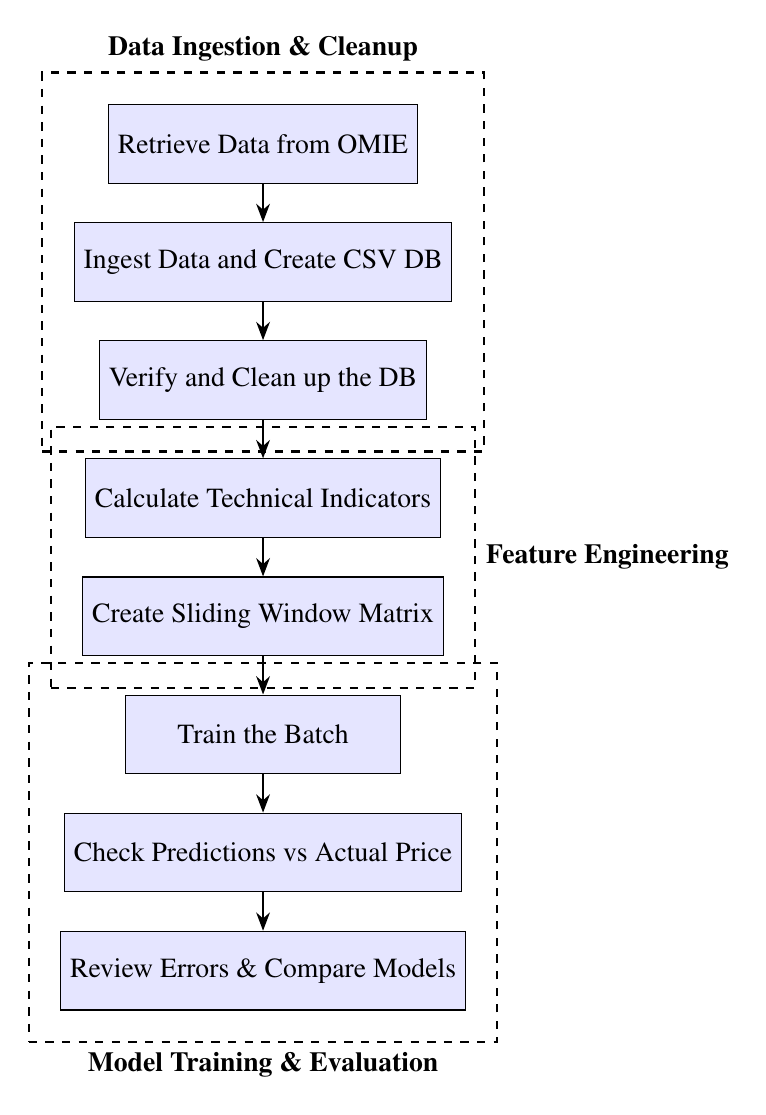
\begin{tikzpicture}[node distance=1.5cm]
    
    % Styles
    \tikzstyle{process} = [rectangle, minimum width=3.5cm, minimum height=1cm, text centered, draw=black, fill=blue!10]
    % \tikzstyle{process} = [rectangle, minimum width=3.5cm, minimum height=1cm, text centered, draw=black]
    \tikzstyle{arrow} = [thick,->,>=Stealth]

    % Nodes
    \node (retrieve) [process] {Retrieve Data from OMIE};
    \node (ingest) [process, below of=retrieve] {Ingest Data and Create CSV DB};
    \node (clean) [process, below of=ingest] {Verify and Clean up the DB};
    \node (indicators) [process, below of=clean] {Calculate Technical Indicators};
    \node (matrix) [process, below of=indicators] {Create Sliding Window Matrix};
    \node (train) [process, below of=matrix] {Train the Batch};
    \node (predict) [process, below of=train] {Check Predictions vs Actual Price};
    \node (review) [process, below of=predict] {Review Errors \& Compare Models};

    % Arrows
    \draw [arrow] (retrieve) -- (ingest);
    \draw [arrow] (ingest) -- (clean);
    \draw [arrow] (clean) -- (indicators);
    \draw [arrow] (indicators) -- (matrix);
    \draw [arrow] (matrix) -- (train);
    \draw [arrow] (train) -- (predict);
    \draw [arrow] (predict) -- (review);

    % Group boxes
    \node[draw=black, thick, dashed, fit={(retrieve)(ingest)(clean)}, inner sep=0.4cm, label=above:{\textbf{Data Ingestion \& Cleanup}}] {};
        \node[draw=black, thick, dashed, fit={(indicators)(matrix)}, inner sep=0.4cm, label=right:{\textbf{Feature Engineering}}] {};
    \node[draw=black, thick, dashed, fit={(train)(predict)(review)}, inner sep=0.4cm, label=below:{\textbf{Model Training \& Evaluation}}] {};

    \end{tikzpicture}
    \caption{Data Processing Pipeline}
    \label{fig:data_processing_pipeline}
\end{figure}


% Intro and preparation for the actual body of work
\section{Prior Set Up and Configuration}
% \textbf{Prior Set Up and Configuration}

Before getting into the system explanation, there are some important pre-requisites that must be met in order to run the project. The project was developed and tested with Python 3.13 \cite{python3.13}, so for any recreation of the project, it is highly recommendable to use the same version. For additional assurance of reproducibility, and as a universal best practice for Python development, it is strongly advisable to set up a new virtual environment \cite{python_venv}. Alternatively, another system that would achieve the same goal of reproducibility, and dependency conflict avoidance would be the use of Miniconda \cite{conda}. This project uses the built in in Python module \textit{venv}, with which a virtual environment can be easily created and configured with the project dependencies following the steps in \textit{\hyperref[app:appendix_a_env_setup]{Appendix A}}.

% Should I write this in the background part, or the software and licenses part?
The chosen libraries were specifically selected to aid in the development of the project. Most of the project was written in Jupyter Notebooks, which are dependent on the \textit{ipykernel} package. To aid in the retrieval of the data, the \textit{requests} package was used to execute HTTP requests. For the manipulation of the data points, \textit{pandas} was used to house the data structures, \textit{numpy} for mathematical operations using arrays, and the \textit{ta} technical analysis library was used to compute the technical indicators. Finally the machine learning algorithms were provided by the \textit{scikit-learn} library.

Following the completion of this prior set up required for the project, the next sections will detail in depth the different steps involved in the system pipeline.

% Three main blocks: create three sections


% Data ingestion and cleanup
\section{Data Preparation: Ingestion and Cleanup}

% General idea as a summary of what is needed in this part??

% 1. Download of OMIE data (only section independent of the whole system)
The first step in any data preparation process would be to retrieve the raw data from the original source, in this case this means downloading it from the OMIE. It is publicly available data easily discoverable through their webpage \cite{omie_datos}. The data collected was all that was initially available towards the end of 2024, with some extraordinary retrievals done later on in 2025 to further complete the set with more data points.

In this scenario, it meant retrieving data from 2018 onward. While for the 5 first years available the data was self contained in a compressed archive file, the rest from 2023 to our current 2025 was not. This meant manually downloading each daily data file. In order to streamline this process, a short Python script was created to build the necessary URIs to retrieve the files with an HTTP GET request.

The Python script in \textit{\hyperref[app:appendix_b_data_scrapping]{Appendix B}} was written with modularity in mind for ease of use. It firstly creates the filenames according to the OMIE's file naming convention, inserting them into a list. This list is essential to successfully build the URIs with which the HTTP GET request will be made. Finally the function \verb|download_files(urls)| makes the request, retrieving the files.

% 2. Data Organization
The newly downloaded raw data was manually organized into its corresponding folder per year. An example filename is the following: \small{\verb|marginalpdbc_20230102.1|}. This is an important organizational step for the ingestion of the data, as the next procedure involves a script that iterates through these folders, identifying all files that start with \small{\verb|marginalpdbc_|}, and parsing them into an easier to use form, a Pandas DataFrame \cite{dataframe}.

% 3. Initial Data Cleanup
When a valid file is identified while iterating through the \textit{year} folders, the script reads its content. It will perform some cleanup steps, such as removing the first and last rows which are a standard header and footer across all files. It then parses the remaining data, which is separated by semicolons, into a Pandas DataFrame for that specific day. It will name the columns to \textit{Year}, \textit{Month}, \textit{Day}, \textit{Hour}, \textit{MarginalPT} (Portuguese Energy Price), and \textit{MarginalES} (Spanish Energy Price). It will also filter out any rows where the \textit{Year} column is not a number, ensuring data integrity. The columns are then converted to their appropriate data types, \textit{integers} for date/time components and \textit{}{floats} for marginal prices. Each processed daily dataset is then temporarily stored in a list.

% 4. Retention of only the relevant data: Datetime and MarginalES
After processing all the individual files, the script concatenates all the daily data from the list of DataFrames into a single, comprehensive DataFrame. It will then construct a \textit{Datetime} column built from the \textit{Year}, \textit{Month}, \textit{Day}, and \textit{Hour} columns. It will also handle some peculiar cases where an \textit{Hour} value of 25 might appear (likely due to daylight savings time zone adjustments) by converting it to 0. This \textit{Datetime} column is then set as the DataFrame's index. Finally, it removes the individual date and hour columns as well as the \textit{MarginalPT} column, leaving only the \textit{MarginalES} as the primary target feature, along with the \textit{Datetime} index.
% también es feature... (para hacer predicciones la variable target en días pasados es feature)

% 5. Final Data Cleanup and Storage
This clean and combined dataset will be saved as a CSV file for ease of use, \small{\verb|raw_data.csv|}. The script then performs further data cleanup by reloading the \small{\verb|raw_data.csv|}, and sorting it by \textit{Datetime}, saving it as \small{\verb|processed_data.csv|}. The whole process concludes by verifying the completeness of the hourly timestamps within the processed data, generating the full range of hourly timestamps that should be there, and checking for any discrepancies. If no missing timestamps are found, it confirms successful data processing; otherwise, it reports the missing timestamps, indicating an error in the data collection or processing.

For the previous in-depth explanation, you may find in \textit{\hyperref[app:appendix_c_ingestion_n_cleanup]{Appendix C}} the of Python script that was created for the desired data ingestion and cleanup tasks.

After completing this ingestion and cleanup process, the dataset will be reduced to just the 14\textsuperscript{th} hour data point. The code in \textit{\hyperref[app:appendix_d_dataset_reduction]{Appendix D}} will create a the final database file, which will house the singular \textit{Datetime} value, and the \textit{MarginalES} data point.

To aid in the predictions, the dataset is enhanced with more features. We can calculate a variety of different features to aid the training of the model. These can range from simple variables such as the day of the week, the month of the year, or if that day is a weekend or not, to more complex, such as technical indicators. By adding these auxiliary features derived from \textit{technical analysis}, we can further expand the context that our models will be able to learn from, ideally improving their prediction accuracy capabilities.

To generate these additional features, and the strategically chosen technical indicators, the main database \small{\verb|processed_data.csv|} is read into a DataFrame that will be progressively expanded with new feature columns. The resulting DataFrame will be saved to a secondary database \small{\verb|ta_metrics_hour_14.csv|}. The code in \textit{\hyperref[app:appendix_e_ta_feature_calculations]{Appendix E}} is an example of the process that was employed to calculate the different indicators, using the open source Python library \textit{ta} \cite{ta-lib}.


% The Feature Matrix for the Sliding Window Approach
\section{Feature Matrix Creation}

% Theory behind feature matrices:
The creation of a \textit{feature matrix} is a key step in the process of training any machine learning model. In this context, the objective is to structure historical energy price data into a form that can be used to effectively train models to predict future prices. The correct transformation of the raw time-series to form our feature matrix is critical for this process. The intent of building the feature matrix consists on creating one unique matrix that can be used across any desired model. The feature matrix denoted as $\mathit{X}$, represents the input data used to train the model, while the target / label vector $\mathit{y}$ contains the values the model is intended to learn how to predict.

% For a given time series, we will map the price values chronologically where x_i:
% \begin{equation*}
% {T} = \begin{bmatrix}
% t_1 \\
% t_2 \\
% t_3 \\
% t_4 \\
% t_5 \\
% t_6
% \end{bmatrix} = \begin{bmatrix}
% x_1 \\
% x_2 \\
% x_3 \\
% x_4 \\
% x_5 \\
% x_6
% \end{bmatrix}
% \end{equation*}

The simple feature matrix of an example time series of 6 price values $x_1$ through to $x_6$ can be represented as:
\begin{equation*}
{X} = \begin{bmatrix}
x_1 & x_2 & x_3 \\
x_2 & x_3 & x_4 \\
x_3 & x_4 & x_5
\end{bmatrix}, \quad
{y} = \begin{bmatrix}
y_1 \\
y_2 \\
y_3
\end{bmatrix}
\end{equation*}

Where each row of $\mathit{X}$ corresponds to a sliding window of past values, and its corresponding label $\mathit{y}$ is the value that follows that window, which would be the actual energy price for the current day:
\begin{align*}
y_1 &= x_4 \\
y_2 &= x_5 \\
y_3 &= x_6
\end{align*}

This setup reflects the temporal dependency in the time-series data, where future values are predicted based on a certain number of past observations. This approach allows the machine learning models to "learn" these implicit patterns in the considered sliding window, enabling them to better predict the next value.

Incorporating technical analysis indicators into the feature matrix introduces additional information such as moving averages or the rate of change calculated over historical price windows, These enrich the model’s inputs and are added as extra columns to the feature matrix:

\begin{equation*}
{X} = \begin{bmatrix}
x_1 & x_2 & x_3 & ta_{11} & ta_{21} & \cdots & ta_{n1}\\
x_2 & x_3 & x_4 & ta_{12} & ta_{22} & \cdots & ta_{n2}\\
x_3 & x_4 & x_5 & ta_{13} & ta_{23} & \cdots & ta_{n3}
\end{bmatrix}
\end{equation*}

Where:
\begin{itemize}
    \item $x_i$ are raw price values from previous time steps,
    \item $n$ is the number of indicators,
    \item $ta_{ji}$ is the value of the $j$-th technical indicator computed based on the last price input of row $i$, i.e., $x_{i+2}$ in this 3 previous days example.
\end{itemize}

The target / label vector will remain unchanged:
\begin{equation*}
\mathbf{y} = \begin{bmatrix}
y_1 \\
y_2 \\
y_3
\end{bmatrix}
\end{equation*}

% The thought process behind our sliding window approach has to do with the data and the following: The dataset is NOT stationary. The data is not independent and identically distributed.
This design is motivated by the nature of the energy market data, which is \textit{non-stationary}, as the statistical properties of electricity prices (e.g. mean, variance) change over time due to evolving supply and demand dynamics, regulatory interventions, and renewable energy contributions. Since the dataset has inherent \textit{temporal dependencies}, as prices are typically dependent on recent values, making the assumption of independent and identically distributed (i.i.d.) samples invalid. The aim is to identify \textit{local trends}, implementing a sliding windows approach allows the model to capture short-term patterns and trends without requiring the data to be stationary.

By using a sliding window mechanism, the models will be trained on a continuous stream of overlapping data segments. This not only increases the number of training samples, enhancing generalization, but also aligning with the real-world scenario of forecasting the next value based on a recent history of observations. The ultimate aim is to build the feature matrix using the sliding window approach to provide a robust and flexible representation of temporal data, allowing traditional machine learning models to operate more effectively in a domain typically reserved for time-series-specific methods.

The Python Script found in \textit{\hyperref[app:appendix_f_simple_feature_matrix]{Appendix F}} contains the code necessary to create the simple feature matrix, which was initially generated based off \textit{MarginalES} values, with the desired sliding window width for that training batch. For an example run we can retrieve from the database a sliding window of 6 days:
\begin{small}
\begin{verbatim}
               Datetime  MarginalES
187 2019-01-01 14:00:00       65.88
188 2019-01-02 14:00:00       63.16
189 2019-01-03 14:00:00       66.70
190 2019-01-04 14:00:00       69.17
191 2019-01-05 14:00:00       64.00
192 2019-01-06 14:00:00       64.86
\end{verbatim}
\end{small}

For which the resulting simple feature matrix is the following:
\begin{small}
\begin{verbatim}
print(X_simple)
0      1      2
0  65.88  63.16  66.70
1  63.16  66.70  69.17
2  66.70  69.17  64.00

print(y_simple)
0    69.17
1    64.00
2    64.86
\end{verbatim}
\end{small}

The simple feature matrix function was later modified and extended to incorporate additional feature columns such as the focus of our proposal, the technical indicators. These are the previously calculated features in order to expand the context our models will be able to train with. The script located in \textit{\hyperref[app:appendix_g_extended_feature_matrix]{Appendix G}} demonstrates the flexible and auto-adaptable nature code, suitable for any number of inputted features (columns) obtained from the secondary feature enhanced database, which includes the additional technical indicators.

Furthermore, for an example run of the matrix creation with the technical indicators we can retrieve the extended database and select the same date range as in the previous example for comparison. Where  we may observe an identical matrix to the earlier one, extended laterally to include the new feature columns, such as the technical indicators and additional \textit{"Datetime"} related context:
\begin{small}
\begin{verbatim}
print(X_extended)
   price_t-3  price_t-2  price_t-1      SMA_3   SMA_5      SMA_7     SMA_14  \
0      65.88      63.16      66.70  65.246667  64.974  63.842857  64.975000   
1      63.16      66.70      69.17  66.343333  66.026  64.490000  65.401429   
2      66.70      69.17      64.00  66.623333  65.782  65.434286  65.330000   

      SMA_30     SMA_90    SMA_180  ...     RSI_30  BB_Width_7  BB_Width_14  \
0  64.886000  65.044333  67.227333  ...  50.823486   17.871701    15.638302   
1  64.988333  65.038667  67.272889  ...  52.153121   21.198596    16.528083   
2  64.947333  65.184222  67.267611  ...  49.268675   11.634263    16.685668   

      STD_7    STD_14    STD_30    STD_90  month  day_of_week  is_weekend  
0  3.080999  2.636139  2.620006  4.626188    1.0          3.0         0.0  
1  3.691585  2.804414  2.726835  4.620755    1.0          4.0         0.0  
2  2.055690  2.828060  2.732317  4.369895    1.0          5.0         1.0

print(y_extended)
0    69.17
1    64.00
2    64.86
\end{verbatim}
\end{small}


% Training of each model with the Matrix
\section{Machine Learning Model Training}

There are multiple strategies that can be implemented for an effective model training, depending on if the dataset is \textit{stationary} or not. An \textit{incremental} approach can be taken when de data is  \textit{stationary}, since in this case, the accumulating the data points will benefit the model's training. An \textit{adaptive} approach is in order when the dataset is of \textit{non-stationary} nature. Similar to an exponential moving average, where the newer data holds more weight, while the older data's importance is progressively minimized, this investigation's models were trained with a sliding window approach, where the older data points are cut off. This training method "forgets" the earliest values as they are no longer relevant in order to make the latest prediction, which is is the case in the energy prices database

The idea behind the previously introduced \textit{adaptive learning} approach is simple, we will create a 1 day step loop across the complete time series. A finite set of days will be used in training each model, with each instance being utilized for one single prediction. The training phase will consist on searching the optimal sliding window of days, with the calculated set of features. In each iteration, the model will be trained with a set feature matrix, and will then be fed with the next feature row to test its prediction abilities.

Continuing with our previous example, the model will be trained with the feature matrix $\mathit{X}$.

% Training Diagram
\begin{figure}[H]
    \centering
    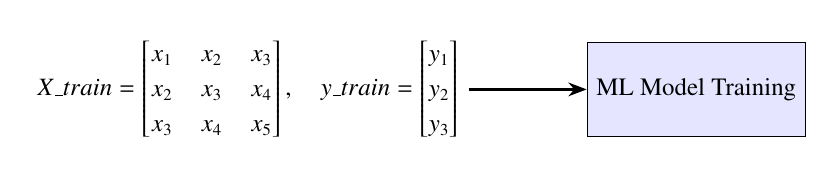
\begin{tikzpicture}[
        node distance=2cm and 1.5cm,
        every node/.style={font=\small},
        model/.style={rectangle, minimum width=2.5cm, minimum height=1.2cm, text centered, draw=black, fill=blue!10},
        % model/.style={rectangle, minimum width=2.5cm, minimum height=1.2cm, text centered, draw=black},
        arrow/.style={thick,->,>=Stealth}
    ]

    % Nodes
    \node (input) {$
                    {X\_train} =
                        \begin{bmatrix}
                            x_1 & x_2 & x_3 \\
                            x_2 & x_3 & x_4 \\
                            x_3 & x_4 & x_5
                        \end{bmatrix}, \quad
                    {y\_train} =
                        \begin{bmatrix}
                            y_1 \\
                            y_2 \\
                            y_3
                        \end{bmatrix}
                   $};
    \node (model) [model, right=of input] {ML Model Training};

    % Arrows
    \draw [arrow] (input) -- (model);

    \end{tikzpicture}
    \caption{Simple Training Example}
    \label{fig:train_example}
\end{figure}

In order to predict a new value, for example, $\hat{y_4}$, the model will be fed the next row of feature values \{$x_4, x_5, x_6$\}, where $x_6$ will be our last known value, $y_3$.

% Predicting Diagram
\begin{figure}[H]
    \centering
    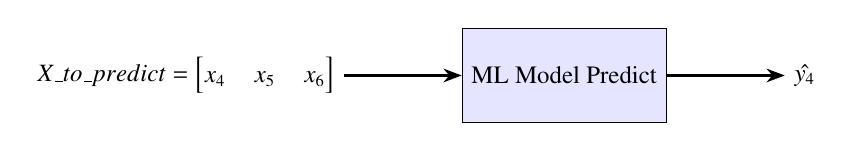
\begin{tikzpicture}[
        node distance=2cm and 1.5cm,
        every node/.style={font=\small},
        model/.style={rectangle, minimum width=2.5cm, minimum height=1.2cm, text centered, draw=black, fill=blue!10},
        % model/.style={rectangle, minimum width=2.5cm, minimum height=1.2cm, text centered, draw=black},
        arrow/.style={thick,->,>=Stealth}
    ]

    % Nodes
    \node (input) {$
                    {X\_to\_predict} =
                        \begin{bmatrix}
                            x_4 & x_5 & x_6
                        \end{bmatrix}
                   $};
    \node (model) [model, right=of input] {ML Model Predict};
    \node (output) [right=of model] {$\hat{y_4}$};

    % Arrows
    \draw [arrow] (input) -- (model);
    \draw [arrow] (model) -- (output);

    % % Annotation
    % \node [below=0.7cm of input] {\footnotesize $x_6 = y_3$};

    \end{tikzpicture}
    \caption{Simple Prediction Example}
    \label{fig:pred_example}
\end{figure}

% - Linear Regression: Linear combination of every feature
The model selection for the project will consist of three models: the Linear Regressor, the Lasso Regressor, and the Random Forest Regressor. The first of the models, the \textit{Linear Regressor} \cite{linear_regression} will serve as our baseline. This model assumes that the target variable can be approximated as a linear combination of the input features. With the sliding window approach it will be possible to test multiple configurations of the model, but in comparison to the other tested models, it does not have an explicitly tunable hyperparameter.

% - Lasso Regression: Linear model that penalizes unused features
Our second model, the \textit{Lasso Regressor} \cite{lasso_regression}, extends the linear model by introducing \textit{L1 regularization}, meaning it has the ability to penalize unused features. This penalty encourages sparsity in the feature weights, effectively performing a feature selection. By tuning its hyperparameter \textit{alpha} ($\alpha$), we can modify the strength of the regularization. This can potentially improve the model's performance, by reducing overfitting, possibly improving its generalization capabilities. To optimize its predictive accuracy, we will later experiment across a variety of \textit{alpha} hyperparameter values.

% - Random Forest: - Non-linear and soft on peaks
The third and final model considered in this investigation, is the \textit{Random Forest Regressor} \cite{random_forest_regressor}, an ensemble learning method based on decision trees. During training, it constructs multiple decision trees, and aggregates their outputs by averaging the regression tasks. We can tune its training process by adjusting parameters such as \verb|n_estimators| (number of trees) and the \verb|max_depth| (maximum depth of each tree). Its output will be averaged, which can be a limiting factor for its predictions, since even if it is capable to learn more complex patterns than the aforementioned models, it will tend to underestimate extreme peak values. This model has been included as a non-linear alternative to validate the performance of the linear models and capture more complex relationships within the data.

Regardless of the chosen model, the training strategy will be as follows: After importing the complete dataset, we will define the number of days you want to include in the sliding window. This determines how many days from the time series will be included in the training. At the same point, we will select the desired number of previous days to be included in the feature matrix as columns. Depending on the selection of the sliding window size, there will be more or less models to train.

After initializing the variables where the predictions, actual values, and their time stamps will be stored at, the training loop will begin. Here, a new model will be trained per iteration as seen in Figure \ref{fig:train_example}, and a new value will be predicted as seen in Figure \ref{fig:pred_example}. Once all models and predictions have been processed, the \small{\verb|prediction_df|} DataFrame will be available for evaluation of the predictive precision of the training loop.

To finalize the system description, the example script found in \textit{\hyperref[app:appendix_h_example_basic_training_process]{Appendix H}} shows in Python code the basic function definition for our sliding window training process, in which any given model could be used. However, it is a basic example that does not test multiple sliding windows, nor consider any hyperparameter tuning. This will be covered in the following section, in the dedicated \textit{Experimentation} chapter.



% Chapter 4 - Experimentation
\chapter{Experimentation}
This chapter presents all of the relevant information pertaining the experimentation phase of the project. We review the specifics of the data that was dealt with, and explain the decisions taken for the preparation of such data, and the training of the different machine learning models employed. We review all of the results of the different models, and discuss in depth the different set-up variations for the models.


\section{Data Description} % Data Description – OMIE data
The data that was used for this project was exclusively publicly available information, published by the OMIE. The data retrieved from their website \cite{omie_datos} for this project takes the following shape:

\begin{small}
\begin{verbatim}
MARGINALPDBC;
2018;01;01;1;28.1;6.74;
2018;01;01;2;33;4.74;
2018;01;01;3;32.9;3.66;
...
2018;01;01;22;28.1;21.95;
2018;01;01;23;28.1;23.52;
2018;01;01;24;27.6;16.35;
*
\end{verbatim}
\end{small}

We can understand and interpret this format following the OMIE's guide: \textit{Modelo de Ficheros para la distribución pública de Información del mercado de electricidad 1.35} \cite{omie_formatos_2024}. In page number 67, chapter 6.18 we may find the following information regarding the encoding format for the information:

\begin{small} % so a bit more text can appear
\begin{verbatim}
6.18 Precios marginales del mercado diario (MARGINALPDBC)

Fichero con los precios marginales del Mercado Diario para cada una de
las horas.
Nombre del fichero: marginalpdbc_aaaammdd.v donde aaaammdd
corresponde a la fecha de sesión y v es la versión del fichero.

Descripción de los campos:
CAMPO DESCRIPCIÓN VALORES VÁLIDOS
Año Año I4 – 20XX
Mes Mes I2 – 1 a 12
Día Día I2 – 1 a 31
Hora Hora I2 – 1 a 25
MarginalPT Precio marginal zona Portuguesa F8.2 – -99999.99 a 99999.99
MarginalES Precio marginal zona Española F8.2 – -99999.99 a 99999.99
\end{verbatim}
\end{small}

From this data description we can obtain the following column names: \textit{Año, Mes, Día, Hora, MarginalPT} and \textit{MarginalES}. As a proof of concept, in this investigation we will be focusing on a single time slot, simplifying the data, from multiple data points per day, to a single one. We are exclusively interested in the value of the last column, \textit{MarginalES}, and specifically the row pertaining the 14\textsuperscript{th} hour of each day.
% another option 14$^{th}$


% Explain some more about the data distribution.
\noindent \textbf{Dataset Analysis and Interpretation}

After the data is ingested into the database, we can inspect the time series by visualizing the data points, and the data distribution, including the mean, median, and mode values of the dataset.

\begin{figure}[H]
    \centering
    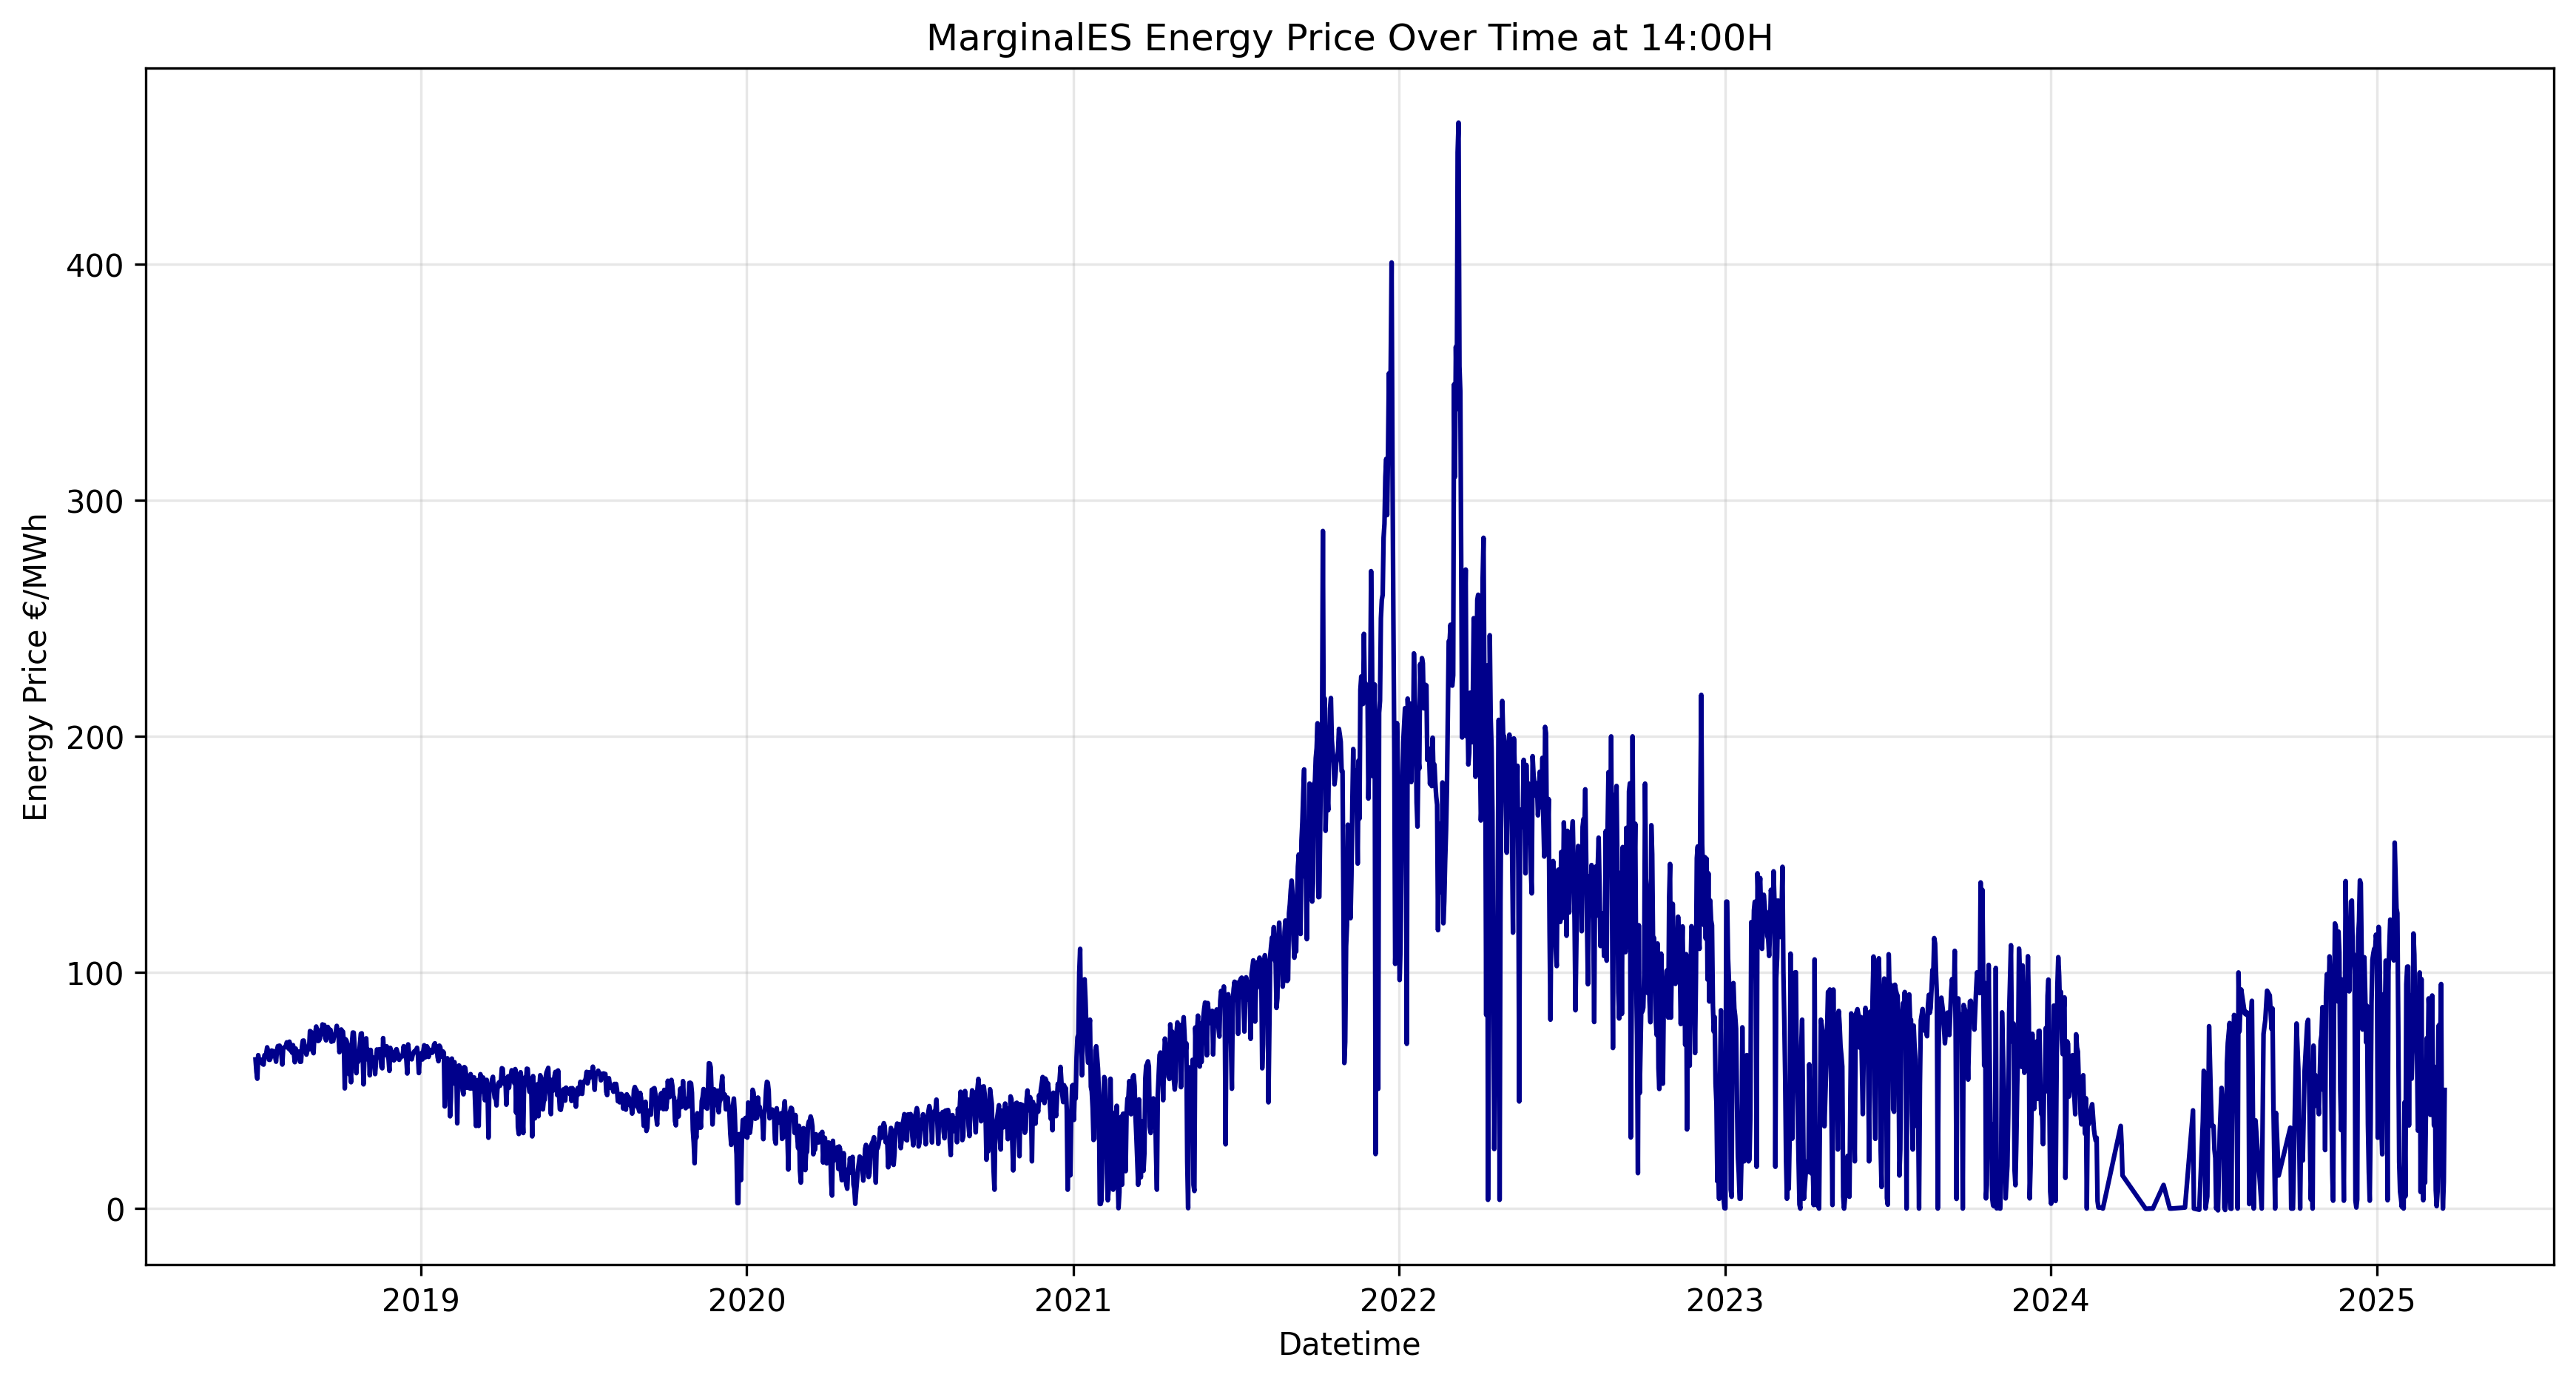
\includegraphics[width=\textwidth]{imagenes/marginal_energy_price_plot.png}
    \label{fig:complete_time_series}
    \caption{MarginalES Price Time Series at 14:00H}
\end{figure}

A visual inspection of the dataset reveals that the observations that form the time series does not meet the assumptions of being independently and identically distributed (i.i.d.) and is also clearly non-stationary. The series exhibits temporal dependencies, with strong correlations between consecutive observations. The aforementioned \textit{sliding window} approach will be the key to correctly processing this time series with techniques usually meant for working with i.i.d. datasets, 

% Estás trabajando desde el principio con series temporales, y lo que haces es adaptar herramientas y técnicas diseñadas para trabajar con datos iid (que no forman una serie temporal) para encontrar una solución a tu problema, que está definido en términos de series temporales.

The energy prices show distinct periods, starting with relatively stable prices around 50-70 €/MWh from 2018 to late 2020, followed by growing volatility and a dramatic surge beginning in late 2021 that peaks at 460 €/MWh in 2022. This price escalation coincides with the escalating tensions, and eventual start of the war between Russia and Ukraine in February 2022, which severely disrupted European natural gas supplies and created unprecedented energy market volatility.

Since natural gas is a crucial input for electricity generation, this geopolitical crisis directly impacted electricity prices by disrupting the matching of supply and demand in OMIE's daily market, where gas-fired power plants often set the marginal price. The subsequent gradual decline in 2023-2024 reflects market adaptation with alternative supply arrangements, and a reduced gas dependency, though prices remain elevated compared to pre-war levels.

These clear shifts in behavior over time show that the data is not \textit{stationary}, as the average values, variability, and overall distribution change across different periods. Because of this, it makes sense to use an \textit{adaptive} sliding window approach, where the model is regularly retrained on the most recent data. This helps it stay up to date with the latest trends and better handle the ups and downs of a changing energy market.

\begin{figure}[H]
    \centering
    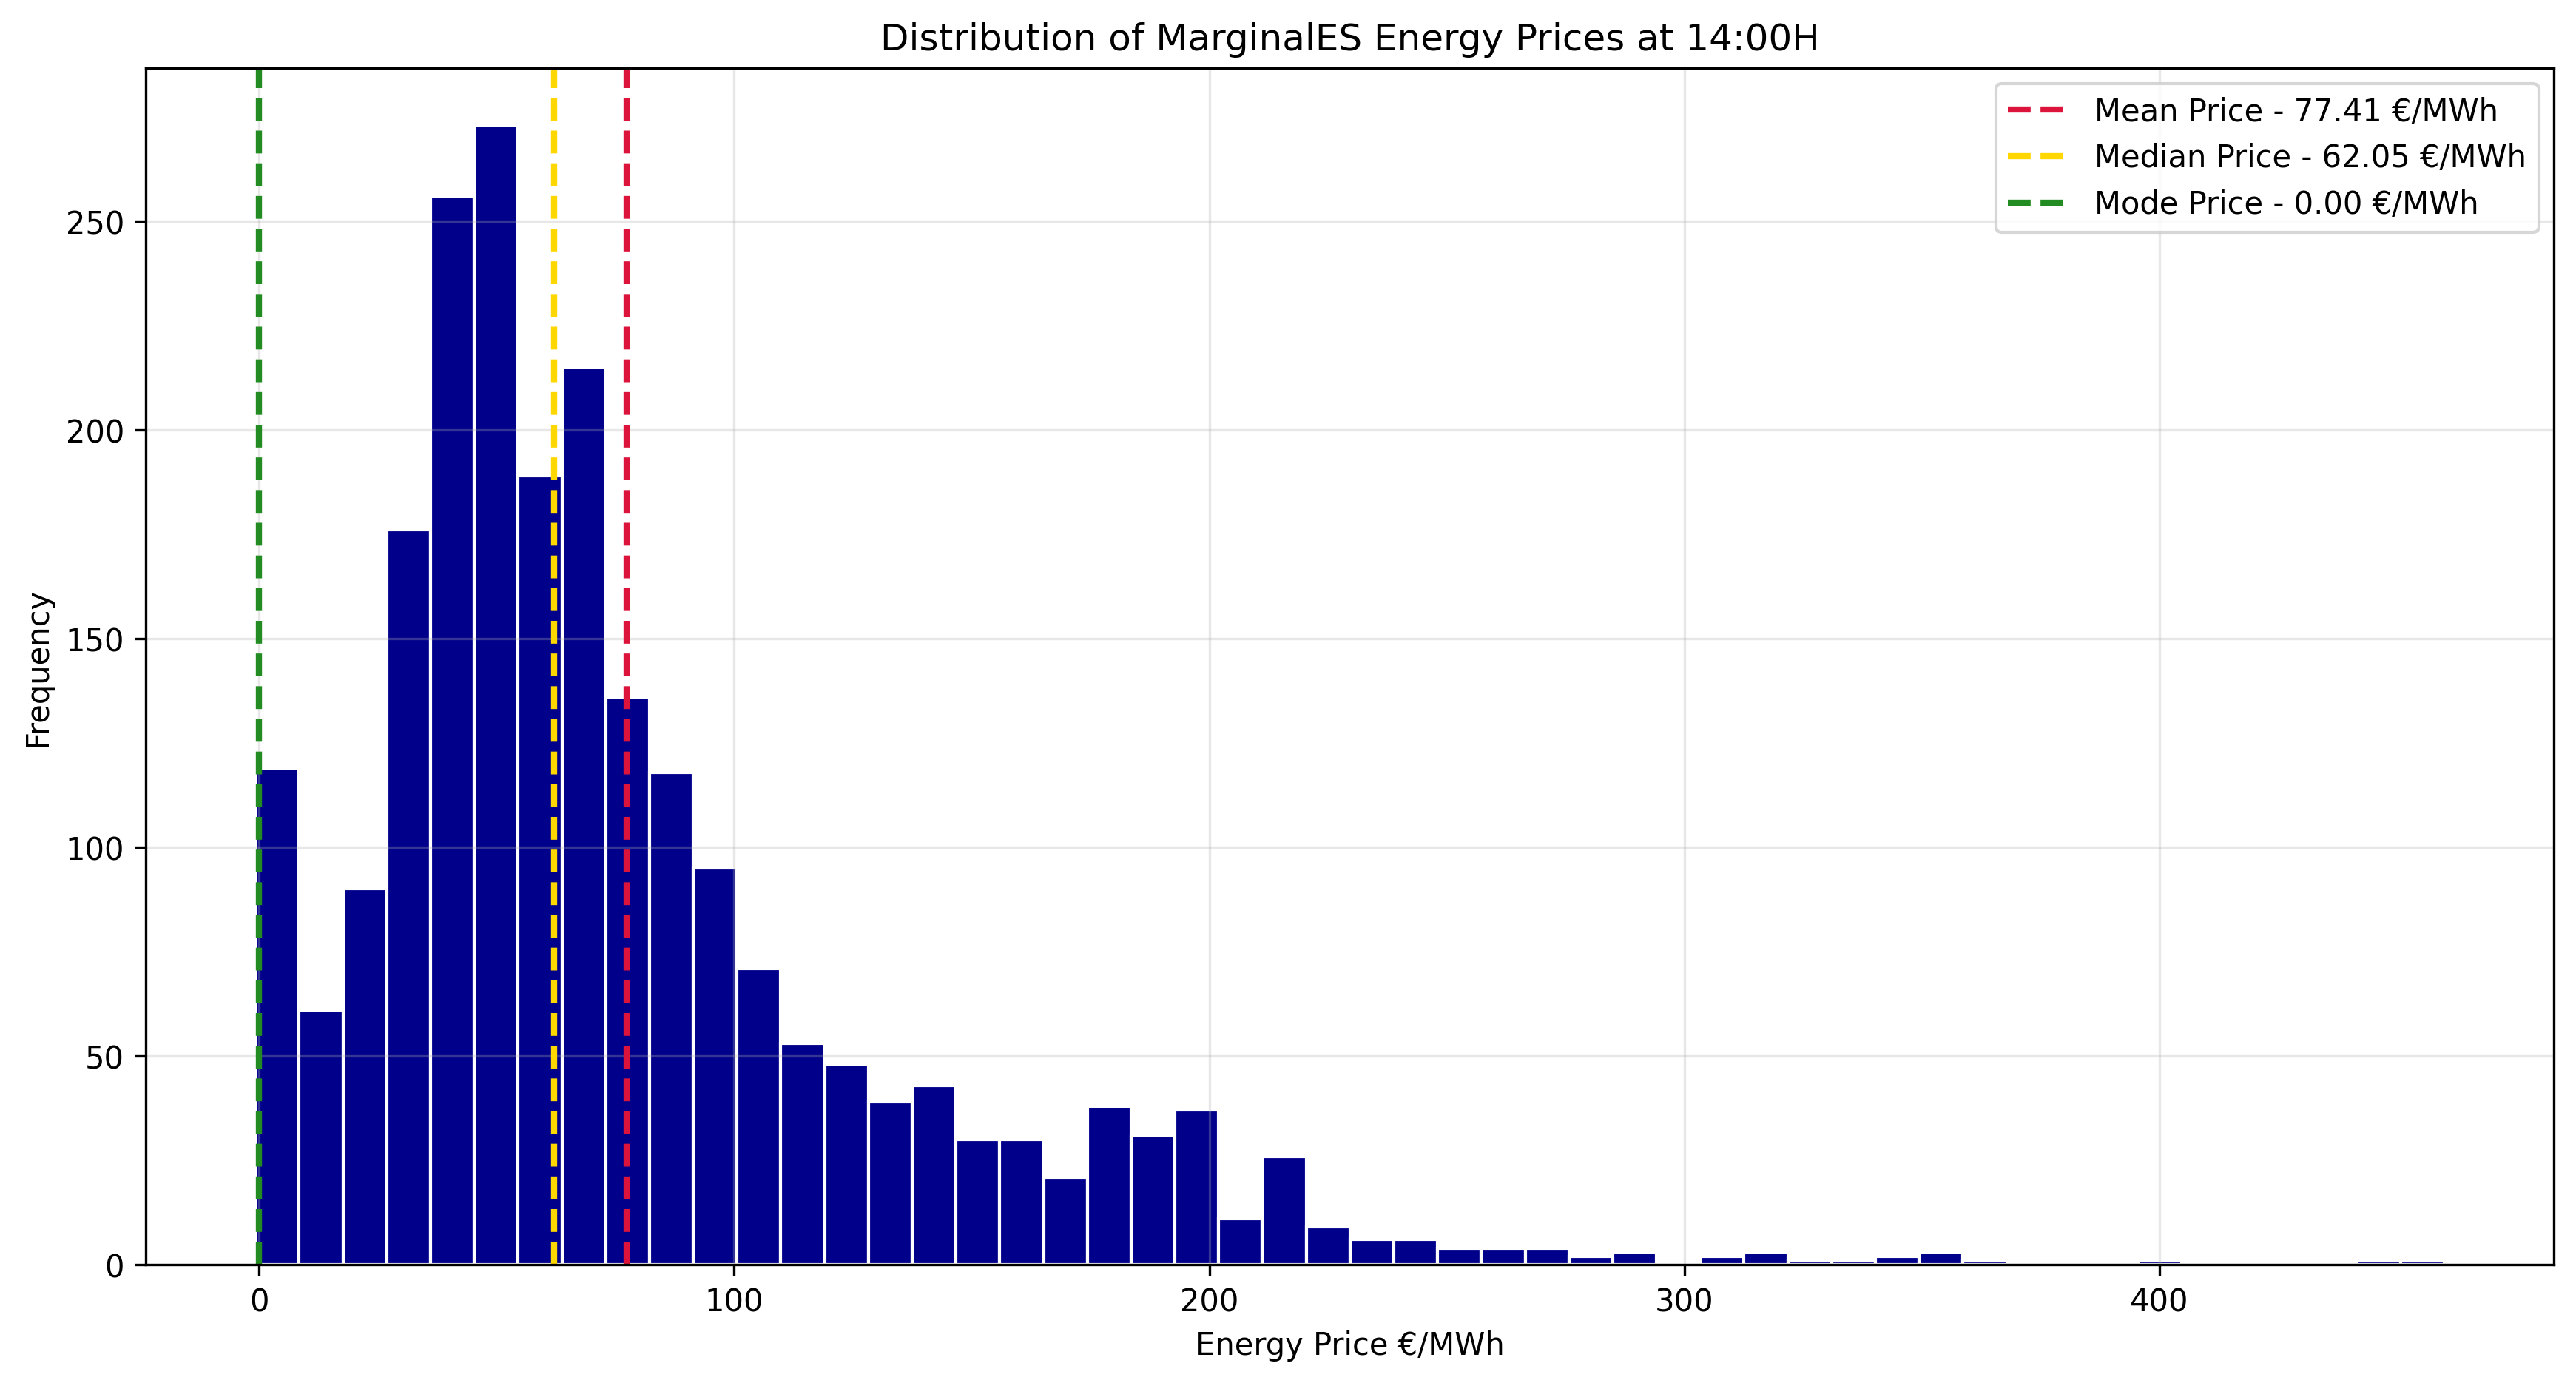
\includegraphics[width=\textwidth]{imagenes/marginal_energy_price_distribution.png}
    \label{fig:data_distribution}
    \caption{MarginalES at 14:00H Data Distribution, Including Mean, Median and Mode Values}
\end{figure}

An interesting observation to comment upon is the mode value, which as seen in the graph, is zero. This can be attributed to the selected hour of the day for our dataset being 14:00H, which is usually around the time when the sun will be at its highest point in the sky, marking the peak production time for solar photovoltaic energy in Spain. And since Spain has an extremely large amount of solar power plants, this means that there will be an overabundance of energy, and therefore the price will plummet down to 0.

In general, the time series posses a high correlation between the prices of neighboring days, with seasonal variations, slow and progressively changing the price. The task at hand for the models is to figure out the best fit to the time series for any of the proposed sliding window configurations.


\section{Model Set Up Explanation}

To assess the predictive performance of the different models introduced earlier, a series of controlled experiments were implemented. In order to successfully run these experiments, the previously explained model training was modified and extended. The most significant modification was the addition of support for batch training across multiple \textit{temporal window configurations}, referring to the combination of the key parameters common to all models: \verb|sliding_window| and \verb|lag_price_window|. These parameters are crucial to identify the best performing temporal windows for each model's training.

For each model, a baseline version was first trained and tested exclusively using the raw time series data. This will serve as the primary comparison benchmark to evaluate the added value of the feature engineering process across each of the models.

For \textit{linear regression}, the focus was solely on evaluating its baseline performance against the engineered features. This was done across a variety of temporal window configurations, without any further hyperparameter adjustments, since linear regression does not include tunable parameters

The \textit{lasso regression} experiments expanded upon the different temporal window configuration training batches, by also testing across multiple values of its regularization hyperparameter $\alpha$. In this modelThe objective was to assess its impact on feature selection and model generalization.

For our final model, a similar was done for the \textit{Random Forest}, not only testing across multiple temporal window configurations, but also exploring different combinations of tree depth (\verb|max_depth|) and the number of leaf nodes (\verb|n_estimators|) to control model complexity and prevent overfitting.

The following sections will present the specific configurations and numerical values used for each of the tested parameters across the different models. This includes the temporal window parameters, as well as the hyperparameters specific to each model. The experiments and their performance evaluations presented in the next sections are entirely based on the models trained using these specific parameter configurations.


% Tabla unica comparando todas las iteraciones de cada technologia? y luego una conjunta con la mejor de todo (Si me hace falta mas, pues al apendice)
\section{Results of the Model Experiments}
% - Show best set of results for each model in graphs (both baseline and feature engineered)

% - Create one unique table comparing the best iteration between each technology

% - Comment and compare the models in a simple and understandable manner - talk about the effect of feature engineering, about the best sliding window, and the impact of tuning the model hyperparameters 

This section presents the best results obtained across the different models. It provides a general overview of the performance potential of each mode, highlighting the impact of both feature engineering and hyperparameter tuning on the final outcomes.

All of the following results presented correspond to the 99\textsuperscript{th} percentile of prediction errors, meaning the top 1\% of the largest errors were excluded. This was chosen in order to fairly represent model performance while minimizing the influence of extreme outlier predictions that are likely caused by isolated model errors.

The considerations taken to decide the top performing model were simple and focused on practical predictive performance. A custom score was created that averages out the ranking of the 4 metrics, the model with the higher rank will be our top performer.

This process was created to take into equal account the value of the four computed error metrics. The MAE, MSE and ES-like metric will be ranked by ascending order, meaning the lower the metric, the higher the rank. In contrast, the $R^2$ will be ranked by descending order, as the top value for it is 1, so the closer to it, the higher the rank.

% Role
% Metric to emphasize

% Best overall accuracy
% MAE

% Outlier control
% MSE

% Model stability
% ES-like

% Overall goodness of fit
% R²

% Mean Absolute Error (MAE) was selected as the primary metric for model comparison, as it provides the error in the same units as the target values (€/MWh). It is a directly interpretable measure of the average prediction error, making it particularly suitable for energy price forecasting. 

% Mean Absolute Error (MAE) was selected as the primary metric for model comparison, as it provides a direct and interpretable measure of average prediction error, making it particularly suitable for energy price forecasting where typical deviations carry operational significance. Additionally, an Expectation Shortfall-like metric was incorporated to account for worst-case scenarios by evaluating the average error among the largest residuals. This ensures that the selected model not only performs well on average but also maintains robustness under less favorable conditions, minimizing the risk of large, costly prediction failures. Mean Squared Error (MSE) and the coefficient of determination (R²) were also calculated and monitored to provide supplementary insights into model fit and variance explanation, but were not the primary criteria in determining the best-performing configuration.


\noindent \textbf{Linear Regression}

Starting with the testing, the first model used will be linear regression. It does not have any tunable hyperparameters, so no manual model optimization was done. The training batches were limited to testing different sliding windows.

The first experiment developed was a baseline training run, limited to just the the raw time series, without any feature engineering. The results of the top three models are as follows:

\begin{table}[H]
	\caption{Best Baseline Regression Models}
	\centering
	\begin{tabular}{|P{2cm}|P{2cm}|P{1.8cm}|P{1.8cm}|P{1.8cm}|P{1.8cm}|}
		\hline
		\textbf{Sliding Window} & \textbf{Lag Window} & \textbf{MAE} & \textbf{MSE} & \textbf{R\textsuperscript{2}} & \textbf{ES-like} \\
		\hline
		30 & 1 & 15.195 & 519.777 & 0.842 & 16.513 \\
		\hline
		30 & 2 & 15.472 & 530.800 & 0.841 & 16.902 \\
		\hline
		90 & 1 & 15.817 & 544.762 & 0.838 & 17.101 \\
		\hline
	\end{tabular}
\end{table}

The plot for the best performer is the following:
% Graph showing the performance
\begin{figure}[H]
    \centering
    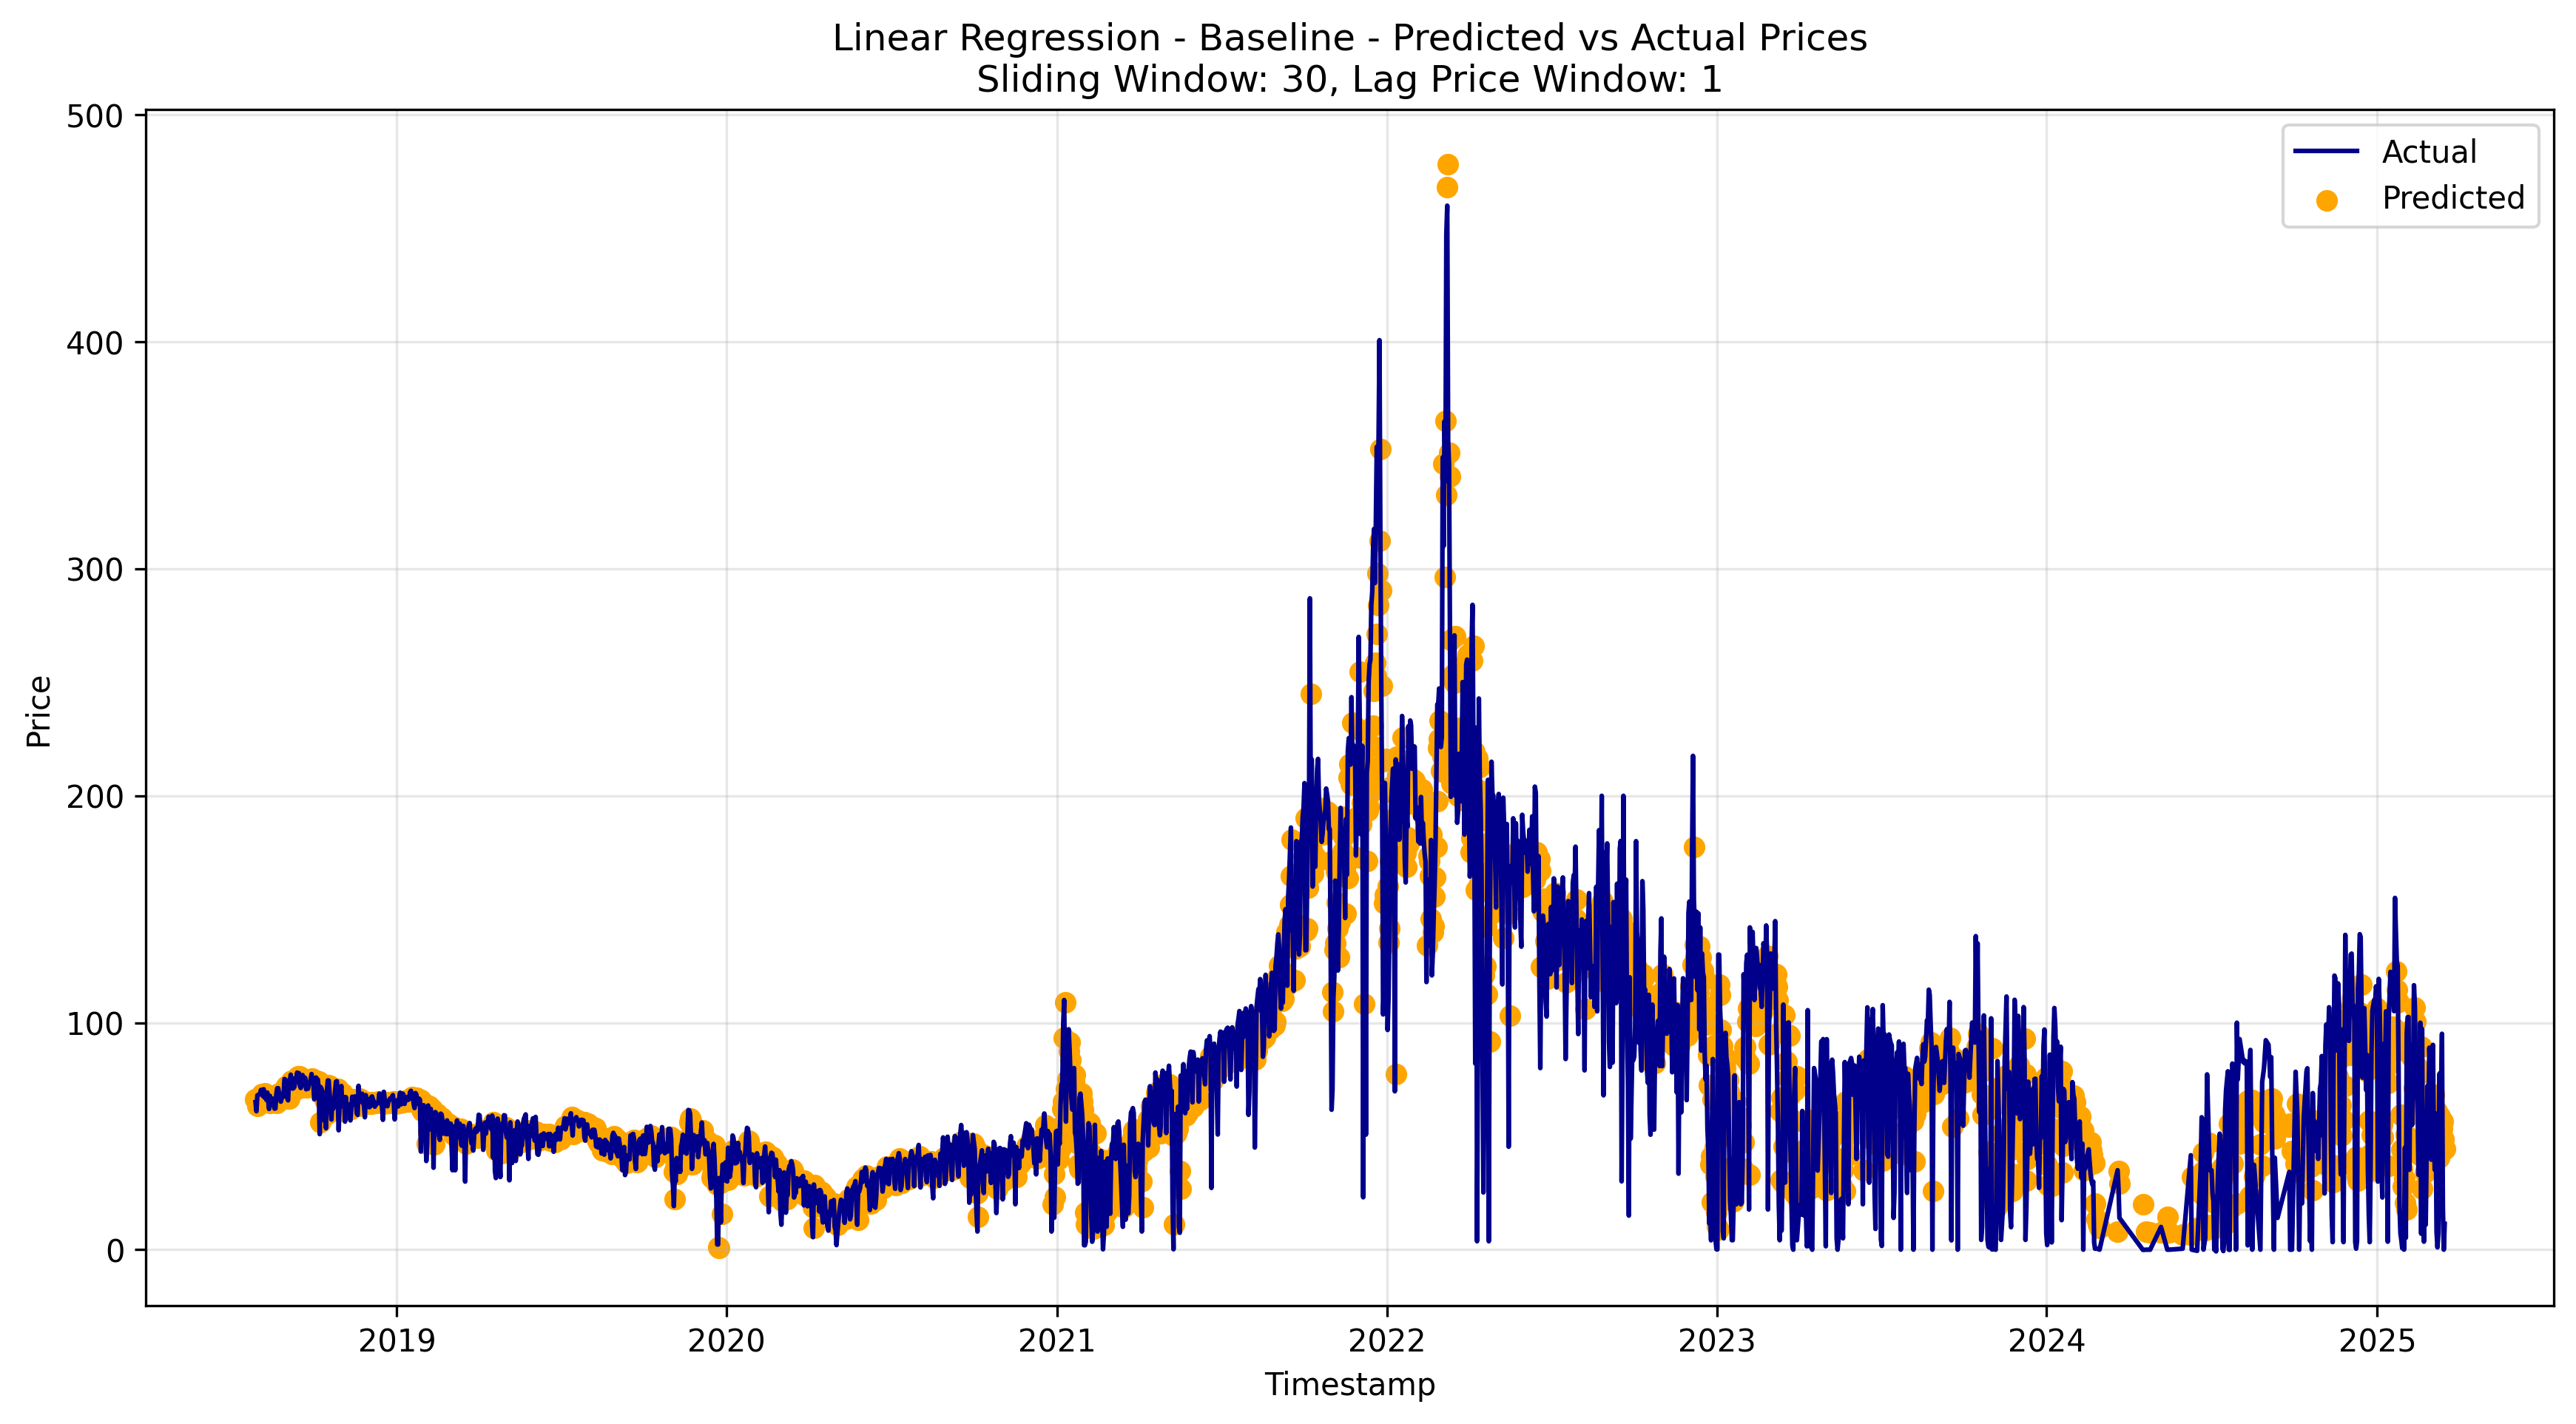
\includegraphics[width=\textwidth]{imagenes/regression_baseline_best_model.png}
    \label{fig:regression_baseline_best_model}
    \caption{Best Linear Regression Baseline Model}
\end{figure}

A visual inspection indicates that even with these me


The next experiment consists of using the more complex feature matrix, which includes the calculated technical indicators. This will review the potential improvements and variations of the feature engineering training run, in comparison to the baseline run. The best result for the feature engineeing batch is the following:

\begin{figure}[H]
    \centering
    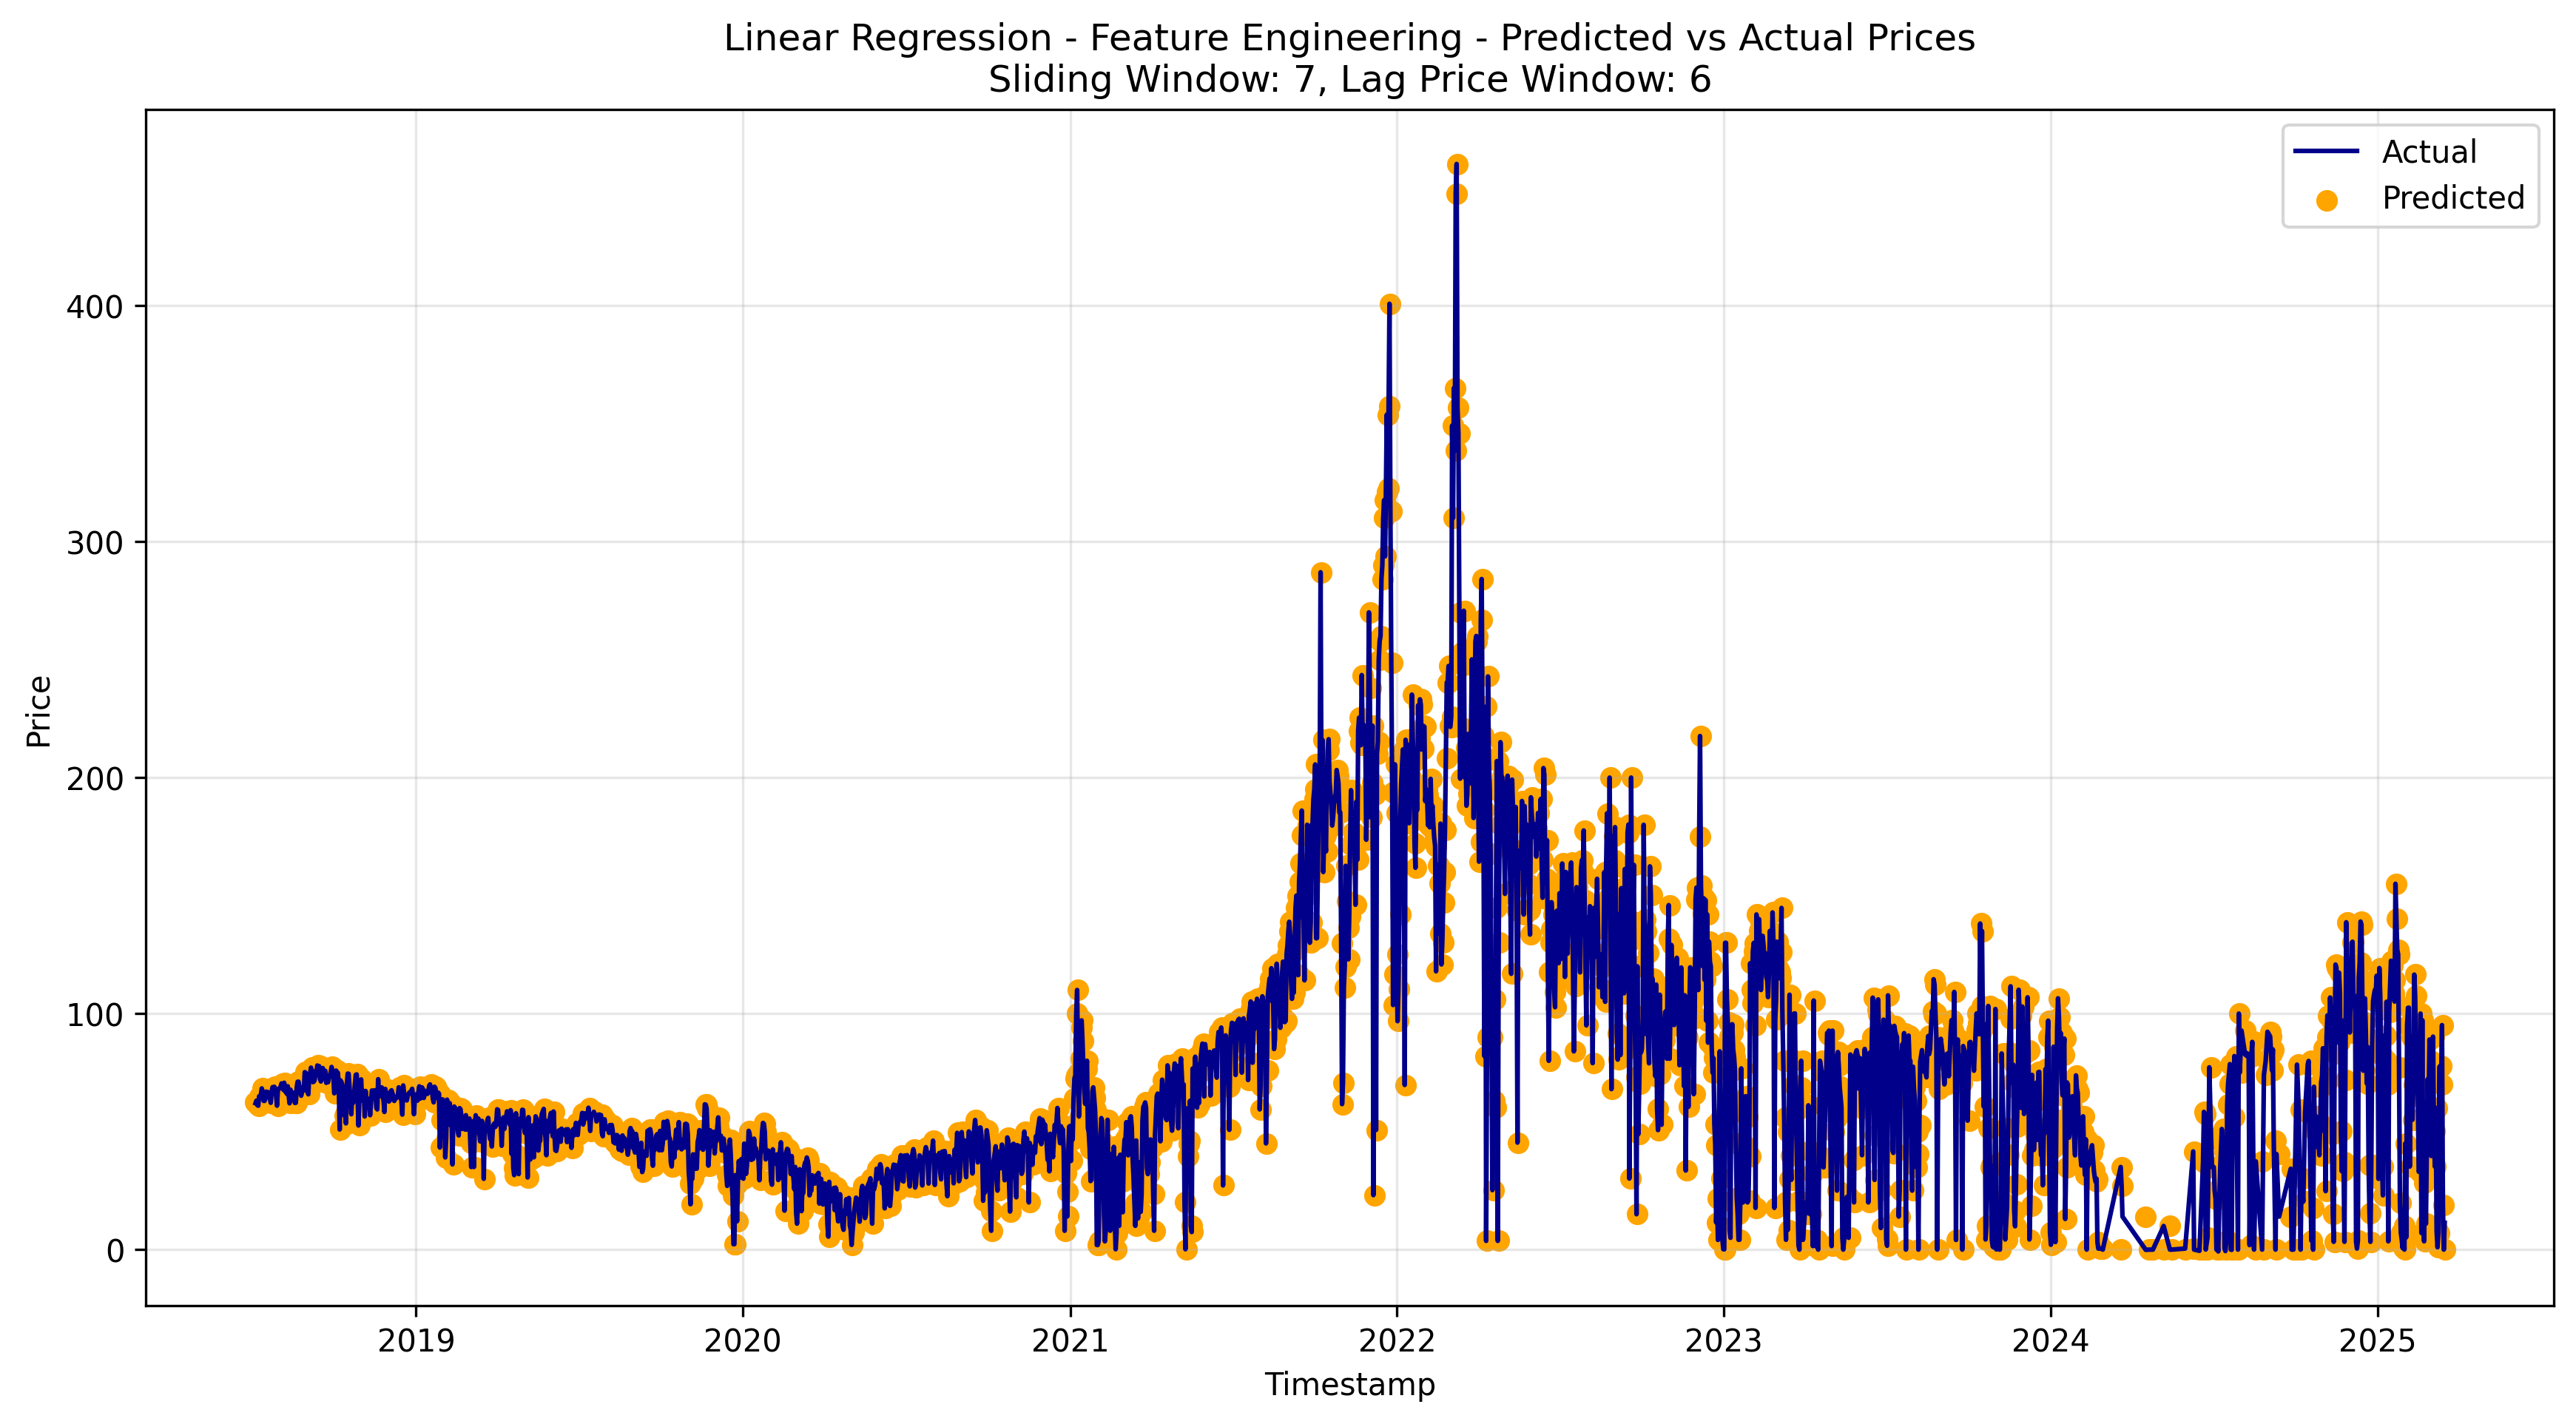
\includegraphics[width=\textwidth]{imagenes/regression_fe_best_model.png}
    \label{fig:regression_fe_best_model}
    \caption{Best Linear Regression Feature Engineering Model}
\end{figure}


% Table showing best configurations

The following example displays the configuration for \verb|sliding_window = | and \verb|lag_price_window = |:

Image of data series across percentiles:

Image of r2 metric to show how on target predictions were:

\noindent \textbf{Lasso Regression}

For the second model considered in this project, Lasso regression, a linear model that penalizes unused features was chosen. Lasso does have a tunable hyperparameter \textit{alpha}, enabling manual model optimization. A selection of parameter values will be tested in every sliding window iteration, noting down the \textit{alpha} value that renders the result with the minimum error to the actual data point.


% COPILOT EXPLAINS FE graphs looking identical
% The two plots look almost identical because both models are essentially learning the same underlying pattern from your feature engineering approach. Here's why:

% Same Feature Engineering = Same Information
% Both models are using:

% Sliding Window: 7 - Same historical price data (7 previous time points)
% Lag Price Window: 6 - Same lagged price features
% Same target variable - Next period's price
% Since the feature engineering creates the same input representation for both models, they're working with identical information about price patterns and trends.

% Linear vs Regularized Linear
% Linear Regression: Finds the best linear combination of your engineered features
% Lasso Regression: Also finds a linear combination but with L1 regularization
% With your high alpha value (1000.0), Lasso is applying strong regularization, but the underlying linear relationship between your features and the target appears to be:

% Strong and consistent - The regularization isn't dramatically changing the predictions
% Well-captured by linear methods - Your feature engineering has created features that have a clear linear relationship with the target
% Why This Happens
% Your sliding window and lag features are capturing the autocorrelation and momentum in the price series effectively. Since financial time series often have strong short-term momentum patterns, both linear methods converge to very similar solutions when given the same well-engineered features.

% This suggests your feature engineering is working well - you've created informative features that clearly represent the underlying price dynamics.

\noindent \textbf{Random Forest}

Soft on peaks - tune hyperparameters like n estimators, max depth, etc.

The last model that was experimented with was the Random Forest regressor. The two main parameters that we will focus on tuning are the number of trees in the forest (\small{\verb|n_estimators|}) and the maximum depth of the tree branches (\small{\verb|max_depth|}). Similar to the training process of the Lasso Regressor, for every sliding window iteration each combination of parameters will be tested. Likewise, we will save the combination of parameters with the best result, with the least error to the actual data point.

Concluding the main results overview, the following table presents the best performing run of each model:
\begin{table}[H]
	\caption{Best Performing Configuration for Each Model}
	\centering
	\begin{tabular}{|P{2.5cm}|P{1.8cm}|P{1.8cm}|P{3.2cm}|P{1.5cm}|P{1.5cm}|}
		\hline
		\textbf{Model} & \textbf{Sliding Window} & \textbf{Lag Window} & \textbf{Hyperparameters} & \textbf{MSE} & \textbf{R\textsuperscript{2}} \\
		\hline
		Linear Regression & - & - & - & - & - \\
		\hline
		Lasso Regression & - & - & $\alpha = -$ & - & - \\
		\hline
		Random Forest & - & - & max\_depth= -, n\_estimators= - & - & - \\
		\hline
	\end{tabular}
\end{table}

Discuss the results:

- Did the FE work?

- Is there any common SW or LW parameters?


\section{Discussion} % of the results
- This will be the final explanation of the results. The one I would give to a colleague of mine, with full details on how every run performed, and how the batches stack up against each other.

- Create one table per model comparing across the other not displayed iterations:

Example table:
\begin{table}[htbp]
\centering

\begin{tabular}{|c|c|c|c|c|c|c|}
\hline
\textbf{Window Configuration} & \textbf{Percentile} & \textbf{Data Points} & \textbf{R²} & \textbf{MSE} & \textbf{MAE} \\
\hline
\multirow{5}{*}{\begin{tabular}[c]{@{}c@{}}Sliding Window: 30\\Lag Price Window: 1\end{tabular}} 
& 100 & 2229 & 0.800 & 688.93 & 16.34 \\
& 99 & 2206 & 0.842 & 519.78 & 15.20 \\
& 95 & 2117 & 0.884 & 335.49 & 12.92 \\
& 85 & 1894 & 0.937 & 161.33 & 9.49 \\
& 75 & 1672 & 0.961 & 86.95 & 7.20 \\
\hline
\multirow{5}{*}{\begin{tabular}[c]{@{}c@{}}Sliding Window: 30\\Lag Price Window: 2\end{tabular}} 
& 100 & 2229 & 0.787 & 733.78 & 16.73 \\
& 99 & 2206 & 0.842 & 530.80 & 15.47 \\
& 95 & 2117 & 0.883 & 347.52 & 13.21 \\
& 85 & 1894 & 0.935 & 171.37 & 9.78 \\
& 75 & 1672 & 0.958 & 91.62 & 7.41 \\
\hline
\multirow{5}{*}{\begin{tabular}[c]{@{}c@{}}Sliding Window: 90\\Lag Price Window: 1\end{tabular}} 
& 100 & 2169 & 0.799 & 710.08 & 16.93 \\
& 99 & 2147 & 0.839 & 544.76 & 15.82 \\
& 95 & 2060 & 0.882 & 356.30 & 13.52 \\
& 85 & 1843 & 0.933 & 177.34 & 10.07 \\
& 75 & 1627 & 0.959 & 97.47 & 7.73 \\
\hline
\end{tabular}

\caption{Performance Analysis of Top X Linear Regression Window Combinations by Percentile}
\label{tab:regression_window_combinations}
\end{table}

- Deep dive into the error rates of each run and compare with other iterations/ batches and other models:

MAE, MSE, R2, Percentiles \& Expectation Shortfall-like metric

For Random Forest

% 1. n_estimators (Number of trees in the forest)
%   Description: This is arguably the most important parameter. It determines the number of decision trees that will be built in the forest.
%   Impact:
%       Higher n_estimators: Generally leads to a more robust and stable model, reducing variance and improving generalization performance.
%       Lower n_estimators: Can result in underfitting if too few trees are used, and the model might not capture complex patterns.
%       Computational Cost: Increasing n_estimators also increases training time and prediction time.

% Tuning Tip: Start with a moderately high number (e.g., 100-200) and increase it until the validation error no longer significantly improves.


% 3. max_depth (Maximum depth of each tree)
%   Description: Limits how deep each individual decision tree in the forest can grow.
%   Impact:
%       Higher max_depth (or None - unlimited): Allows trees to be very deep and potentially overfit to the training data. This is often desired for individual trees in a Random Forest, as the ensemble averaging mitigates overfitting.
%       Lower max_depth: Creates shallower, less complex trees, which can prevent overfitting but might lead to underfitting if the model is too simplistic.

% Tuning Tip: While default None often works well for Random Forests due to the ensemble nature, you might experiment with values like 10, 20, or 30 to control complexity if you observe overfitting.

%-------------------



% Chapter 5 - Regulatory Framework (Marco Regulador)
\chapter{Regulatory Framework}
% Not essential for this investigative project because we do not go to market.

In any data-driven project understanding the regulatory landscape is essential. This chapter addresses the legal, ethical, and operational constraints that governed the use of data and software throughout the development of this project. From the data acquisition and pre-processing, to the software deployment and reproducibility, each component aims to comply with relevant national and international standards to ensure a responsible and legal development.


\section{Data Availability}

The dataset used in this project was obtained from the OMIE, a publicly traded company designated as the Iberian energy market operator. This organization publishes the energy market data as part of their legal obligations set by the Spanish CNMC for transparency, aligned with European regulations.

% I need to talk about laws? What data is permissible to use and how. This would be essential for a project that does indeed go to market.
For the purpose of this thesis, which is strictly academic and investigative in nature, Spanish and European regulations allow for the use of publicly available institutional data without requiring additional licenses. This includes data shared under open access or public sector information frameworks, specifically for research, education, or non-commercial work.

However, it is important to note that if the project were to evolve into a commercial application, the legal requirements would change. In such a scenario, additional licensing agreements, permissions for commercial use, and compliance with intellectual property laws may be necessary.

While no personal or sensitive data is used in this project, future developments that incorporate customer or proprietary data would also need to comply with GDPR and ethical standards for responsible AI and data use, especially in markets as sensitive as energy trading.

\section{Software \& Licenses}

This project was developed using a combination of open-source and proprietary software tools. In the context of regulatory and legal frameworks, the selection and usage of these tools are not only technical decisions, they also bear implications related to licensing compliance.

To ensure transparency and reproducibility, all core dependencies have been documented. Where applicable, licensing schemes have been reviewed to ensure compatibility with both academic and industrial research standards.

For clarity, the software tools have been categorized into two distinct parts: required software to reproduce the project, and optional tools to enhance the development workflow.

\noindent \textbf{Required Software:}
\begin{itemize}
    \item Python: Primary programming language used throughout the project. Python is open source under the Python Software Foundation License \cite{python}.
    
    \item Pandas: Data manipulation library, distributed under a variety of permissive open-source licenses \cite{pandas}.
    
    \item NumPy: Numerical computing library, distributed under its own open-source license \cite{numpy}. 
    
    \item Scikit-learn: Machine learning library, used for model training and evaluation. \cite{scikit-learn}.
    
    \item ta (Technical Analysis) Library: Used for calculating financial indicators to aid in the time series analysis. It is available under the MIT license, a permissive open-source license \cite{ta-lib}.
    
    \item Matplotlib: Used for data visualization, distributed under a permissive open source license \cite{matplotlib}.
    
    \item macOS: Closed-source operating system on which development was performed. Its usage is subject to commercial a licensing agreement by Apple Inc. \cite{macos}.
\end{itemize}

\noindent \textbf{Optional Software:}
\begin{itemize}
    \item Git: Open-source version control system licensed under GPLv2, used for code tracking and collaboration \cite{git}.

    \item Git: Open-source distributed version control system, used for code tracking and collaboration \cite{git}.
    
    \item GitHub: Repository hosting platform for Git repositories. Though it hosts open-source projects, GitHub itself is a proprietary service governed by its own Terms of Service \cite{github}
    
    \item Visual Studio Code: Open-source code editor under the MIT license, provided by Microsoft \cite{vscode}.
    
    \item Visual Studio Code Extension: Microsoft Data Wrangler: A proprietary extension that provides pandas.DataFrame visualization capabilities during development \cite{VSCode_DataWrangler}.

    \item Python Virtual Environment (venv): Used to make the project environment reproducible. It is best practice to create new Python virtual environments for each new project, specially in a production environment where certain versions are required in order for all components to work as intended \cite{python_venv}. An alternative method of dealing with this would be using Conda, and creating with it a new Conda environment \cite{conda}.

    \item Overleaf: Cloud-based LaTeX editor used to write this document. Overleaf is a closed-source platform with cloud-hosting considerations that may have implications under data protection regulations such as the GDPR \cite{overleaf}
    
    \item LaTeX: Open-source typesetting language used to produce the final project document. Licensed under its own LaTeX Project Public License \cite{latex}.

    \item OpenAI ChatGPT, Google Gemini \& Anthropic Claude: closed source large language models used to aid in troubleshooting general coding issues. Licensed under their own respective terms of use. 
\end{itemize}

No sé como comentar el uso de IA:



Relleno o paso de esto: \url{https://uc3m.libguides.com/en/TFG/GenAI} ?

No veo formato para Latex, sólo un word. Igualmente para rellenarlo con: si, la he usado, pero sólo para lo que se permite en el reglamento (la pagina web)... Pues no sé si merece la pena, o cuan de estrictos serán.

En la matriz de evaluacion no figura como obligatoria: \url{https://www.uc3m.es/secretaria-virtual/media/secretaria-virtual/doc/archivo/doc_matriz_evaluacion/eps_matrizevaluacion_tfg_definitiva_nov24__espanol_ingles.pdf}

Simplemente aquí dice que la incluya si la uso: \url{https://www.uc3m.es/ss/Satellite/SecretariaVirtual/es/TextoMixta/1371210936260/Trabajo_de_Fin_de_Grado#defensa}



% Chapter 6 - Socio-economic Environment - Entorno socio-economico
\chapter{Socio-economic Environment}

Energy markets play a central role in modern economies, directly affecting industrial output, consumer costs, and overall economic stability. Electricity is a resource that cannot be easily stored at scale. Its demand fluctuates continuously, and supply must adapt almost instantaneously. As a result, accurate energy price prediction is not just a technical challenge, but a key enabler for operational efficiency, market stability, and policy decision-making.

This project operates within this socio-economic context. Understanding the broader environment highlights its relevance and the potential future applications of the work. The forecasting models developed here could contribute to better-informed decision making across multiple stakeholders, from grid operators and energy producers to regulators, businesses, and end consumers.


% \section{Socio-economic Impact}
\section{Impact}

Why is this relevant?

- Energy Prediction

- Shutdowns

- Price sensitivity

In this project we have


\section{Project Plan}
TODO: Gantt diagram representing time spent in each phase - Design and innovation time frames

\begin{figure}[H]
    \centering
    \begin{ganttchart}[
        x unit=1cm, % width of one month
        y unit chart=0.8cm,
        hgrid,
        vgrid,
        time slot unit=month,
        time slot format=isodate-yearmonth,
        % compress calendar, % what is this / why is it not working?
        bar height=0.6
        ]{2024-09}{2025-06}
    
        \gantttitlecalendar{year, month=shortname} \\
    
        \ganttgroup{Project Phase 1}{2024-09}{2025-01} \\
        \ganttbar{System Design}{2024-10}{2024-12} \\
        \ganttbar{Coding}{2024-12}{2025-01} \\
    
        \ganttgroup{Project Phase 2}{2025-01}{2025-06} \\
        \ganttbar{Results Gathering}{2025-01}{2025-05} \\
        \ganttbar{Redacting the Thesis}{2025-05}{2025-06}
    
    \end{ganttchart}
    \caption{Gantt Diagram of the Project Lifecycle}
    \label{fig:gantt_diagram}
\end{figure}


\section{Budget}
This section will consist of a complete price breakdown of the investigation, consisting of material costs such as the equipment utilized, and the human capital that composed the investigation team. It is notable to highlight that as previously mentioned, no paid license of any sort was obtained for the realization of this project. All of the programs, tools or code, were either \textit{Open Source} or free to use software under exclusive \textit{non-commercial use} licenses.

The most basic requirement for the physical needs of this project is a computer with an desktop operating system. Since the project was written in Python \cite{python}, it would be reasonable to consider it platform agnostic. Any computer capable of running any recent operating system, configured with a recent version of Python would be able to run this project. This includes any of the three most popular desktop operating systems, Windows, macOS and any Linux distribution.

The project was mainly tested using Python 3.13 \cite{python3.13} which does require a recent operating system such as macOS 13 or Windows 10. But as for the project itself, there is no platform, processor architecture, or processing power requirements. In my case, I mainly developed the code in my personal laptop, a 2021 MacBook Pro configured with the ARM M1 Pro chip and 16GB of RAM, running the latest available macOS version at this time, macOS 15 \cite{macos}. This laptop was obtained from a second-hand store circa June 2024, mainly for personal use, but also helping keep the theoretical project costs down.

The following table outlines the specific equipment costs incurred for the development of this investigative project:
\begin{table}[H]
	\caption{Equipment Amortization}
	\centering
	\begin{tabular}{|P{2.8cm}|P{1.8cm}|P{2.5cm}|P{1.5cm}|P{2cm}|P{1.5cm}|}
		\hline
		\textbf{Equipment} & \textbf{Price (€)} & \textbf{Amortization per year (€)} & \textbf{Useful Life (years)} & \textbf{Usage Time (months)} & \textbf{Cost (€)} \\
		\hline
		MacBook Pro M1 Pro & 1250 & 312.5 & 4 & 9.5 & 247.4 \\
		\hline
	\end{tabular}
\end{table}

Regarding the human capital that was required for the successful development of this project, it will consist exclusively on two people. The director of my bachelor's thesis, professor Emilio Parrado Hernández, PhD, as the expert Machine Learning consultant, and myself as a junior software engineer.

The following table displays the estimated hourly rates of each person, the hours dedicated to the project, and the total cost:
            
\begin{table}[H]
	\caption{Human Costs}
	\centering
	\begin{tabular}{|P{4cm}|P{3.5cm}|P{1.8cm}|P{1.5cm}|P{1.5cm}|}
		\hline
		\textbf{Name} & \textbf{Role} & \textbf{Price (€/hour)} & \textbf{Hours} & \textbf{Cost (€)} \\
		\hline
		Emilio Parrado Hernández & Expert ML Consultant (PhD) & 200 & - & - \\
		\hline
		Rodrigo De Lama Fernández & Junior Engineer (Pre-Graduate) & 30 & - & - \\
		\hline
	\end{tabular}
\end{table}

For our final budgeting considerations, other miscellaneous expenses, such as transportation costs to the university for on site meetings with my bachelor's thesis director. Summing up all costs, the following table estimates what this project would have cost to investigate:

\begin{table}[H]
    \caption{Final Cost Breakdown}
    \centering
    \begin{tabular}{|l|r|}
        \hline
        \textbf{Concept} & \textbf{Cost (€)} \\
        \hline
        Direct/Material Costs & 247.4 \\
        Engineering Costs & - \\
        University Carlos III Costs - Expert ML Consultant & - \\
        \hline
        \textbf{Total} & \textbf{-} \\
        \hline
    \end{tabular}
\end{table}



% Chapter 7 - Conclusions
\chapter{Conclusions}
In this investigation we have analyzed in depth an innovative methodology for predictive modeling of energy prices with Machine Learning algorithms, enhanced by the usage of technical analysis indicators in feature engineering, in order to enhance prediction precision. This final chapter will review the general conclusions attained throughout the development of this project's Machine Learning based solution for energy price predictions. It will also discuss potential development paths for future work pertaining the system designed in this investigative project


% Merged into one section only
% \section{Review of the Investigation} % A recap of the project
% \section{Revisiting the Objectives}

\section{Revisiting the Objectives of the Investigation} % Or Project
After finishing the whole project, read it, and reintroduce the objectives to the reader. Remind them of the completion of them

Predicting the prices in an accurate manner using Machine Learning models using feature engineering with technical analysis indicators


\section{Future Work}
% - Less absolute error, and minimizing model error spikes (menos piradas)
% - Better overall precision: better percentile accuracy
There are several promising directions to improve and extend this investigative work. Firstly, future efforts should focus on reducing the overall absolute error of the model, while also addressing the isolated error spikes that occasionally lead to significant deviations in prediction accuracy. Achieving smoother and more stable forecasts would result in better percentile accuracy across the entire distribution of predicted prices.

% - An architecture combining different models and their strengths for a more accurate prediction. Random Forest consistency mixed with the linear model peaks?
Another potential avenue is the development of a hybrid model architecture that combines the strengths of different algorithms. For example, integrating the consistency and robustness of Random Forests with the sensitivity of linear models would potentially enable capturing sharp price variations and peaks, creating a more balanced and accurate predictor.

% - Production application of this project? A commercial app for price prediction
Finally, with further validation and performance tuning, this project could evolve into a production ready system, potentially serving as the foundation for a commercial application capable of providing real-time electricity price forecasts to companies, traders, and consumers seeking to optimize their energy costs.


%----------
%	Bibliography
%----------	

\clearpage
\addcontentsline{toc}{chapter}{Bibliography}

\printbibliography



%----------
%	Appendix
%----------	
\appendix



\chapter* {Appendix A: Project Environment Configuration}
\pagenumbering{gobble} % Appendix pages are not numbered
\label{app:appendix_a_env_setup}

\noindent Create the virtual environment:
\begin{verbatim}
python -m venv .venv
\end{verbatim}

\noindent Activating the new virtual environment:
\begin{verbatim}
in macOS
source .venv/bin/activate

in Windows
.venv\Scripts\Activate.ps1
\end{verbatim}

\noindent To reproduce the exact environment used in the project, a \textit{requirements.txt} file must be created with the following contents:
\begin{verbatim}
ipykernel==6.29.5
matplotlib==3.10.1
numpy==2.2.3
pandas==2.2.3
requests==2.32.3
scikit-learn==1.6.1
ta==0.11.0
\end{verbatim}

\noindent To install the dependencies run:
\begin{verbatim}
pip install -r requirements.txt 
\end{verbatim}



\chapter* {Appendix B: Automated Download of OMIE Raw Data}
\label{app:appendix_b_data_scrapping}

\begin{lstlisting}
import requests
from datetime import datetime, timedelta

# Usage instructions:
    # Set file name to save the filenames to download
    # Set start and end dates

file_path = 'to_download.txt'
start_date = datetime(2023, 1, 1)
end_date = datetime(2025, 3, 18)

# Compose filenames to download
def compose_filenames():
    start_date = start_date
    end_date = end_date
    
    # Generate the entries for the number of days comprehended
    to_generate = (end_date - start_date).days + 1
    entries = []
    for i in range(0, to_generate):  # x days from start to end
        date_entry = start_date + timedelta(days=i)
        entries.append(f'marginalpdbc_{date_entry.strftime("%Y%m%d")}.1')
    
    # Save to a .txt file
    with open(file_path, 'w') as file:
        for entry in entries:
            file.write(entry + '\n')

# Example URI to build
# https://www.omie.es/es/file-download?parents%5B0%5D=marginalpdbc&filename=marginalpdbc_20230102.1
def read_filenames_and_compose_urls(file_path):
    base_url = "https://www.omie.es/es/file-download?parents%5B0%5D=marginalpdbc&filename="
    
    # Read the filenames from the .txt file
    with open(file_path, 'r') as file:
        filenames = [line.strip() for line in file if line.strip()]
    
    # Compose the URLs
    urls = [base_url + filename for filename in filenames]
    
    return urls

def download_files(urls):
    for url in urls:
        # Extract the filename from the URL
        filename = url.split('=')[-1]
        
        # Send a GET request to download the file
        response = requests.get(url)
        
        # Check if the request was successful and write to file
        if response.status_code == 200:
            # Write the content to a file with the extracted filename
            with open(filename, 'wb') as file:
                file.write(response.content)
            print(f"Downloaded {filename}")
        else:
            print(f"Failed to download {filename}")

# Execution
compose_filenames()
urls = read_filenames_and_compose_urls(file_path)
download_files(urls)
\end{lstlisting}



\chapter* {Appendix C: Data Ingestion and Cleanup}
\label{app:appendix_c_ingestion_n_cleanup}

\begin{lstlisting}
import pandas as pd
import os

# Base path to the folder containing the year by year data folders
base_path = '../TFG/data/'

# Initialize an empty list to store DataFrames
all_data = []

# Iterate through each year folder and process all files
for root, dirs, files in os.walk(base_path):
    for file in files:
        # Check if the file starts with 'marginalpdbc_' (ignoring the rest, including the extension)
        if file.startswith('marginalpdbc_'):
            
            # Read the file
            file_path = os.path.join(root, file)
            with open(file_path, 'r', encoding='utf-8') as f:
                lines = f.readlines()

            # Remove the first line (MARGINALPDBC;) and the last line (*)
            data_lines = lines[1:-1]
            
            # Convert the list of semicolon-separated strings into a DataFrame
            daily_data = pd.DataFrame([line.strip().split(';') for line in data_lines])
            
            # Remove trailing ';' from the last column
            if daily_data.shape[1] > 6:
                # Drop empty columns
                daily_data = daily_data.iloc[:, :6]
            
            # Assign column names
            daily_data.columns = ['Year', 'Month', 'Day', 'Hour', 'MarginalPT', 'MarginalES']
            
            # Remove rows with invalid data (in case accidental empty rows, or non-numeric values, get included)
            daily_data = daily_data[daily_data['Year'].str.isdigit()]  # Only keep rows where 'Year' is a number
            
            # Convert the columns to the appropriate data types
            daily_data = daily_data.astype({
                'Year': int, 'Month': int, 'Day': int, 'Hour': int, 'MarginalPT': float, 'MarginalES': float
                })
            
            # Append daily data to the list
            all_data.append(daily_data)

# Concatenate all daily DataFrames into one big DataFrame
full_data = pd.concat(all_data, ignore_index=True)

# Create a datetime column from Year, Month, Day, and Hour
# Adjust the 'Hour' column to deal with the potential 25th hour issue in case of timezone adjustment
full_data['Hour'] = full_data['Hour'].apply(lambda x: 0 if x == 25 else x)
full_data['Datetime'] = pd.to_datetime(full_data[['Year', 'Month', 'Day', 'Hour']], errors='coerce')

# Set the 'Datetime' column as the index
full_data.set_index('Datetime', inplace=True)

# Drop the now unnecessary time columns and 'MarginalPT', as we are focusing on the Spanish market
full_data.drop(['Year', 'Month', 'Day', 'Hour', 'MarginalPT'], axis=1, inplace=True)

# Save the full dataset to a CSV file
full_data.to_csv('../../data/raw_data.csv')

# Post-ingest database cleanup:
# Load and sort the data by the 'Datetime', and save the sorted data to a new file
df = pd.read_csv('../../data/raw_data.csv')
df = df.sort_values(by='Datetime')
df.to_csv('../../data/processed_data.csv', index=False)

# Read the CSV file
df = pd.read_csv('../../data/processed_data.csv')
df['Datetime'] = pd.to_datetime(df['Datetime']) # Parse 'Datetime' column to datetime objects

# Generate the complete range of hourly timestamps
full_range = pd.date_range(start=df['Datetime'].min(), end=df['Datetime'].max(), freq='h')

# Find any missing timestamp
missing_timestamps = full_range.difference(df['Datetime'])

# If successful, print a message
if missing_timestamps.empty:
    print("Data ingestion completed successfully.")

# Else, print an error message
else:
    print("Error: Missing timestamps found. Check the data.")
    print("Missing timestamps:\n missing_timestamps")

    print("Data ingestion completed with errors.")
\end{lstlisting}



\chapter* {Appendix D: Dataset Reduction to the 14\textsuperscript{th} Hour}
\label{app:appendix_d_dataset_reduction}

\begin{lstlisting}
import pandas as pd

# Load the original dataset
data_path = '../../data/processed_data.csv'
df = pd.read_csv(data_path, parse_dates=['Datetime'])

# Define the hour to predict and filter down to the 14:00H data point
hour_to_predict = 14
df_hour = df[df['Datetime'].dt.hour == hour_to_predict].copy()

# Save the final database
df_hour.to_csv("../../data/hour_14_metrics.csv", index=False)
\end{lstlisting}




\chapter* {Appendix E: Technical Analysis Indicators Calculations}
\label{app:appendix_e_ta_feature_calculations}

\begin{lstlisting}
import pandas as pd
import ta  # bukosabino's Technical Analysis Library
import numpy as np

# Load the data
data_path = 'data/processed_data.csv'
df = pd.read_csv(data_path, parse_dates=['Datetime'])

# Reduce dataset to only to the 14th hour
hour_to_predict = 14
df = df[df['Datetime'].dt.hour == hour_to_predict].copy()

# The "window" parameter is measured in days

# Trend-following - SMA and EMA
# Simple Moving Average
df[f'SMA_{3}'] = ta.trend.SMAIndicator(close=df['MarginalES'], window=3).sma_indicator()
df[f'SMA_{5}'] = ta.trend.SMAIndicator(close=df['MarginalES'], window=5).sma_indicator()
df[f'SMA_{7}'] = ta.trend.SMAIndicator(close=df['MarginalES'], window=7).sma_indicator() # past week trend
df[f'SMA_{14}'] = ta.trend.SMAIndicator(close=df['MarginalES'], window=14).sma_indicator()
df[f'SMA_{30}'] = ta.trend.SMAIndicator(close=df['MarginalES'], window=30).sma_indicator() # past month trend
df[f'SMA_{90}'] = ta.trend.SMAIndicator(close=df['MarginalES'], window=90).sma_indicator()
df[f'SMA_{180}'] = ta.trend.SMAIndicator(close=df['MarginalES'], window=180).sma_indicator() # past half year trend

# Exponential Moving Average
df[f'EMA_{3}'] = ta.trend.EMAIndicator(close=df['MarginalES'], window=3).ema_indicator()
df[f'EMA_{5}'] = ta.trend.EMAIndicator(close=df['MarginalES'], window=5).ema_indicator()
df[f'EMA_{7}'] = ta.trend.EMAIndicator(close=df['MarginalES'], window=7).ema_indicator()
df[f'EMA_{14}'] = ta.trend.EMAIndicator(close=df['MarginalES'], window=14).ema_indicator()
df[f'EMA_{30}'] = ta.trend.EMAIndicator(close=df['MarginalES'], window=30).ema_indicator()

# Momentum - Rate of Change (ROC) and RSI
# Rate of Change
df[f'ROC_{3}'] = ta.momentum.ROCIndicator(close=df['MarginalES'], window=3).roc()
df[f'ROC_{5}'] = ta.momentum.ROCIndicator(close=df['MarginalES'], window=5).roc()
df[f'ROC_{7}'] = ta.momentum.ROCIndicator(close=df['MarginalES'], window=7).roc()
df[f'ROC_{14}'] = ta.momentum.ROCIndicator(close=df['MarginalES'], window=14).roc()
df[f'ROC_{30}'] = ta.momentum.ROCIndicator(close=df['MarginalES'], window=30).roc()

# Relative Strength Index
df[f'RSI_{5}'] = ta.momentum.RSIIndicator(close=df['MarginalES'], window=5).rsi() # rapid momentum changes
df[f'RSI_{7}'] = ta.momentum.RSIIndicator(close=df['MarginalES'], window=7).rsi()
df[f'RSI_{14}'] = ta.momentum.RSIIndicator(close=df['MarginalES'], window=14).rsi() # biweekly momentum
df[f'RSI_{30}'] = ta.momentum.RSIIndicator(close=df['MarginalES'], window=30).rsi()

# Volatility - Bollinger Bands Width and Standard Deviation
# BB Width (Bollinger Bands Width)
df['BB_Width_7'] = ta.volatility.BollingerBands(close=df['MarginalES'], window=7, window_dev=2).bollinger_wband()
df['BB_Width_14'] = ta.volatility.BollingerBands(close=df['MarginalES'], window=14, window_dev=2).bollinger_wband()

# Standard Deviation (STD)
df['STD_7'] = df['MarginalES'].rolling(window=7).std()
df['STD_14'] = df['MarginalES'].rolling(window=14).std()
df['STD_30'] = df['MarginalES'].rolling(window=30).std()
df['STD_90'] = df['MarginalES'].rolling(window=90).std()

# Additional contextual features
df['month'] = df['Datetime'].dt.month
df['day_of_week'] = df['Datetime'].dt.dayofweek  # Monday=0
df['is_weekend'] = df['day_of_week'].isin([5, 6]).astype(int)

# Drop missing values generated by rolling calculations
df.dropna(inplace=True)

# Check for NaN or infinity values (specially in ROC)
print("NaN values per column:\n", df.isna().sum())
print("Infinity values per column:\n", df.isin([np.inf, -np.inf]).sum())

# Drop NaN or infinity values and interpolate
df = df.replace([np.inf, -np.inf], np.nan).dropna()
df = df.interpolate()

# Save the dataset with metrics
df.to_csv(f'data/ta_metrics/final_price_ta_metrics.csv', index=False)
\end{lstlisting}



\chapter* {Appendix F: Simple Feature Matrix Function and Example Run}
\label{app:appendix_f_simple_feature_matrix}

\noindent \textbf{Function:}
\begin{lstlisting}
import pandas as pd
import numpy as np

def create_feature_matrix(data, lag_price_window):
    """
    Creates a feature matrix where each row is a sliding window of prices,
    and a corresponding target vector containing the next price value.
    
    Parameters:
    ----------
    - data: DataFrame with 'Datetime' and 'MarginalES' columns
    - lag_price_window: Size of the previous prices sliding window
    
    Returns:
    -------
    - X: DataFrame with sliding windows as rows
    - y: Series with target values (next price after each window)
    """
    # Extract the MarginalES column
    if 'MarginalES' in data.columns:
        prices = data['MarginalES'].values
    else:
        # Assume it's the second column (index 1)
        prices = data.iloc[:, 1].values
    
    # Create empty matrices
    X = np.zeros((len(prices) - lag_price_window, lag_price_window))
    y = np.zeros(len(prices) - lag_price_window)
    
    # Fill the matrices with the sliding windows and targets
    for i in range(len(prices) - lag_price_window):
        X[i, :] = prices[i:i+lag_price_window]  # Window of previous prices
        y[i] = prices[i+lag_price_window]       # Next price after window
    
    # Convert to DataFrame/Series for easier use in training
    return pd.DataFrame(X), pd.Series(y)
\end{lstlisting}

\noindent \textbf{Example run:}
\begin{lstlisting}
import pandas as pd
from utils.matrix_builder import create_feature_matrix

# read data
csv_hour_file = '../data/ta_metrics/final_price_ta_metrics.csv'
simple_df = pd.read_csv(csv_hour_file, parse_dates=['Datetime'])
simple_df = simple_df[['Datetime', 'MarginalES']]

# Sliding window of 6 days
train_start_date = '2019-01-01'
train_end_date = '2019-01-07'

simple_subset = simple_df[(simple_df['Datetime'] >= train_start_date) & (simple_df['Datetime'] <= train_end_date)]

# Number of previous days as columns (features)
lag_price_window = 3

X_simple, y_simple = create_feature_matrix(simple_subset, lag_price_window)
\end{lstlisting}



\chapter* {Appendix G: Extended Feature Matrix Function and Example Run}
\label{app:appendix_g_extended_feature_matrix}

\noindent \textbf{Function:}
\begin{lstlisting}
def create_ta_feature_matrix(dataframe, lag_price_window):
    """
    Creates a sliding window dataset for time series forecasting where each row contains:
    1. A window of historical prices (right-aligned)
    2. Feature values from the most recent point in the window
    3. Target value (next price after the window)
    
    Parameters:
    ----------
    dataframe : pandas.DataFrame
        DataFrame containing at minimum 'Datetime' and 'MarginalES' columns, 
        plus any additional feature columns
    lag_price_window : int
        Number of data points to include in each window of previous prices
        
    Returns:
    -------
    X : pandas.DataFrame
        Features DataFrame with:
        - Historical prices labeled as 'price_t-n' through 'price_t-1'
        - All additional features from the original dataframe
    y : pandas.Series
        Target values (price at time t)
    """
    
    # Input validation
    if lag_price_window < 1:
        raise ValueError("Feature window size must be at least 1")
    if len(dataframe) <= lag_price_window:
        raise ValueError(f"DataFrame must have more rows ({len(dataframe)}) than lag_price_window ({lag_price_window})")
    if 'Datetime' not in dataframe.columns or 'MarginalES' not in dataframe.columns:
        raise ValueError("DataFrame must contain 'Datetime' and 'MarginalES' columns")

    X, y = [], []
    
    # Extract price data and features
    df_prices = dataframe[['Datetime', 'MarginalES']]
    df_features = dataframe.iloc[:, 2:] # Exclude 'Datetime' and 'MarginalES'
    feature_names = df_features.columns.tolist()

    # Create samples from the data
    for i in range(lag_price_window, len(df_prices)):
        # Extract the window for prices as features (right-aligned)
        window = df_prices.iloc[i-lag_price_window:i, 1].values.flatten()
        
        # Extract corresponding feature row (from the most recent point in the window)
        feature_row = df_features.iloc[i-1].values.flatten()

        # Concatenate window prices with feature row
        X.append(np.concatenate((window, feature_row)))
        y.append(df_prices.iloc[i, 1])  # Predict current price

    # Create column names for the prices feature window
    price_columns = [f'price_t-{lag_price_window-i}' for i in range(lag_price_window)]

    # Return DataFrame and Series with proper column names
    X_df = pd.DataFrame(X, columns=price_columns + feature_names)
    y_series = pd.Series(y, name='price_t')
    return X_df, y_series
\end{lstlisting}

\noindent \textbf{Example run:}
\begin{lstlisting}
import pandas as pd
from utils.matrix_builder import create_feature_matrix

# read data
csv_hour_file = '../data/ta_metrics/final_price_ta_metrics.csv'
features_df = pd.read_csv(csv_hour_file, parse_dates=['Datetime'])

# Sliding window of 6 days
train_start_date = '2019-01-01'
train_end_date = '2019-01-07'

feature_subset = features_df[(features_df['Datetime'] >= train_start_date) & (features_df['Datetime'] <= train_end_date)]

# Number of previous days as columns (features)
lag_price_window = 3

X_extended, y_extended = create_expanded_feature_matrix(feature_subset, lag_price_window)
\end{lstlisting}



\chapter* {Appendix H: Example of the Basic Training Process}
\label{app:appendix_h_example_basic_training_process}

\begin{lstlisting}
import pandas as pd
import numpy as np
from utils.matrix_builder import create_feature_matrix

# Import your preferred Machine Learning model here
from model_library import preferred_model

# Load Database
csv_hour_file = '../data/ta_metrics/final_price_ta_metrics.csv'
df = pd.read_csv(csv_hour_file, parse_dates=['Datetime'])

def generic_training(df, sliding_window, lag_price_window, DEBUG):
    """
    Train a machine learning model using a sliding window approach.
    
    Parameters:
    - df: DataFrame containing the dataset with features and target variable.
    - sliding_window: Number of rows to use for training in each sliding window.
    - lag_price_window: Number of previous days to use as features.
    
    Returns:
    - prediction_df: DataFrame containing predictions and actual values.
    """
    if DEBUG:
        print("Debug mode is ON. Detailed output will be printed.")

    # Validate input parameters
    if sliding_window <= lag_price_window:
        raise ValueError("Sliding window must be greater than to the lag price window.")

    training_sliding_window = sliding_window + 1  # +1 to include the next row as the test set

    # Calculate number of sliding window models to train in the dataset
    num_sliding_windows = len(df) - training_sliding_window
    if DEBUG:
        # Training for sliding windows and lag price window
        print(f"Training sliding window size: {training_sliding_window}, lag price window size: {lag_price_window}")
        print(f"Number of rows in the dataset: {len(df)}")

    print(f"Number of models to train: {num_sliding_windows}")

    # Initialize lists to store predictions, actuals, and timestamps
    predictions_list = []
    actuals_list = []
    timestamps_list = []

    model = preferred_model()

    for i in range(num_sliding_windows):
        if DEBUG:
            print(f"Processing sliding window {i + 1}/{num_sliding_windows}...")

        # Ensure we do not exceed the DataFrame length
        if i + training_sliding_window >= len(df):
            break  # Avoid index out of bounds
        
        # Extract the sliding window set, including the next row to use for prediction
        sliding_window_set = df.iloc[i : i + training_sliding_window]

        if DEBUG:
            print(f"Sliding window should have {training_sliding_window} rows, got {len(sliding_window_set)} rows.")
            print(f"Sliding window set:\n{sliding_window_set}")
        
        # Create feature matrix and target variable for training
        X_train, y_train = create_feature_matrix(sliding_window_set, lag_price_window)
        
        if DEBUG:
            print(f"Feature matrix shape: {X_train.shape}, Target variable shape: {y_train.shape}")
            print(f"Feature matrix:\n{X_train.head()}")
            print(f"Target variable:\n{y_train.head()}")

        # Split for training and prediction
        X_train_fit = X_train.iloc[:-1]
        y_train_fit = y_train.iloc[:-1]

        X_to_predict = X_train.iloc[-1:]
        y_to_predict = y_train.iloc[-1]

        if DEBUG:
            print(f"Training features shape: {X_train_fit.shape}, Training target shape: {y_train_fit.shape}")
            print(f"Features to predict shape: {X_to_predict.shape}, Target to predict: {y_to_predict}")

        model.fit(X_train_fit, y_train_fit)
        y_predicted = model.predict(X_to_predict)

        # Add a lower bounds to set extreme negative predictions to 0, assuming prices cannot be negative
        if y_predicted[0] < 0:
            y_predicted[0] = 0

        # Store results
        predictions_list.append(y_predicted[0])
        actuals_list.append(y_to_predict)
        if 'Datetime' in sliding_window_set.columns:
            timestamps_list.append(sliding_window_set.iloc[-1]['Datetime'])
        else:
            timestamps_list.append(i + training_sliding_window - 1)

    # Create final prediction DataFrame
    prediction_df = pd.DataFrame({
        'Timestamp': timestamps_list,
        'Predicted': predictions_list,
        'Actual': actuals_list
    })

    if DEBUG:
        print(f"Final prediction DataFrame:\n{prediction_df.head()}")

    return prediction_df
\end{lstlisting}


\end{document}